% Seminarul 15: Risc sistemic
% Statistica piețelor financiare -- Program de licență, Academia de Studii Economice din București
% GENERAT de latex/build_seminar15.py -- modificați generatorul, nu acest fișier.
% Implicit versiunea pentru studenți; versiunea profesorului este wrapper-ul *_solutions.tex.
\makeatletter\@ifundefined{ifsolutions}{\expandafter\newif\csname ifsolutions\endcsname}{}\makeatother

\newcommand{\coursename}{Statistica piețelor financiare}
\def\sfmlang{ro}
% Preambul comun SFM -- Statistica piețelor financiare / Statistics of Financial Markets (Beamer, 16:9)
% Același design ca MFM. Înainte de % Preambul comun SFM -- Statistica piețelor financiare / Statistics of Financial Markets (Beamer, 16:9)
% Același design ca MFM. Înainte de % Preambul comun SFM -- Statistica piețelor financiare / Statistics of Financial Markets (Beamer, 16:9)
% Același design ca MFM. Înainte de \input{../../latex/preamble} se definește
%   \newcommand{\coursename}{Statistics of Financial Markets}      (EN)
%   \newcommand{\coursename}{Statistica piețelor financiare}       (RO)  și  \def\sfmlang{ro}
% Fișierele .tex se află în EN/Courses, EN/Seminars, RO/Cursuri, RO/Seminarii (două niveluri sub rădăcină).
% Deck-urile sînt generate de latex/build_chapterN.py / build_seminarN.py (vezi latex/sfm_build.py).

\documentclass[9pt, aspectratio=169, t]{beamer}
\providecommand{\coursename}{Statistics of Financial Markets}

% Ensure content fits on slides
\setbeamersize{text margin left=8mm, text margin right=8mm}

%=============================================================================
% THEME AND STYLE CONFIGURATION
%=============================================================================
\usetheme{default}
% Using default theme for clean header/footer control

% Color Palette (matching Redispatch PDF)
\definecolor{MainBlue}{RGB}{26, 58, 110}
\definecolor{AccentBlue}{RGB}{26, 58, 110}
\definecolor{IDAred}{RGB}{205, 0, 0}
\definecolor{DarkGray}{RGB}{51, 51, 51}
\definecolor{MediumGray}{RGB}{128, 128, 128}
\definecolor{LightGray}{RGB}{248, 248, 248}
\definecolor{VeryLightGray}{RGB}{235, 235, 235}
\definecolor{KeynoteGray}{RGB}{218, 218, 218}
\definecolor{SectionGray}{RGB}{120, 120, 120}
\definecolor{FooterGray}{RGB}{100, 100, 100}
\definecolor{Crimson}{RGB}{220, 53, 69}
\definecolor{Forest}{RGB}{46, 125, 50}
\definecolor{Amber}{RGB}{181, 133, 63}
\definecolor{Orange}{RGB}{230, 126, 34}
\definecolor{Purple}{RGB}{142, 68, 173}

% Gradient background (exact Keynote 315° gradient: white to RGB 218,218,218)
\setbeamertemplate{background}{%
    \begin{tikzpicture}[remember picture, overlay]
        \shade[shading=axis, shading angle=315,
        top color=white, bottom color=KeynoteGray]
        (current page.south west) rectangle (current page.north east);
    \end{tikzpicture}%
}
% Fallback solid color for compatibility
\setbeamercolor{background canvas}{bg=}

\setbeamercolor{palette primary}{bg=MainBlue, fg=white}
\setbeamercolor{palette secondary}{bg=MainBlue!85, fg=white}
\setbeamercolor{palette tertiary}{bg=MainBlue!70, fg=white}
\setbeamercolor{structure}{fg=MainBlue}
\setbeamercolor{title}{fg=IDAred}
\setbeamercolor{frametitle}{fg=IDAred, bg=}
\setbeamercolor{block title}{bg=MainBlue, fg=white}
\setbeamercolor{block body}{bg=VeryLightGray, fg=DarkGray}
\setbeamercolor{block title alerted}{bg=Crimson, fg=white}
\setbeamercolor{block body alerted}{bg=Crimson!8, fg=DarkGray}
\setbeamercolor{block title example}{bg=Forest, fg=white}
\setbeamercolor{block body example}{bg=Forest!8, fg=DarkGray}
\setbeamercolor{item}{fg=MainBlue}

% Footer colors (override Madrid theme blue)
\setbeamercolor{author in head/foot}{fg=FooterGray, bg=}
\setbeamercolor{title in head/foot}{fg=FooterGray, bg=}
\setbeamercolor{date in head/foot}{fg=FooterGray, bg=}
\setbeamercolor{section in head/foot}{fg=FooterGray, bg=}
\setbeamercolor{subsection in head/foot}{fg=FooterGray, bg=}

% Bullet styles (apply everywhere including blocks)
\setbeamertemplate{itemize item}{\color{MainBlue}$\boxdot$}
\setbeamertemplate{itemize subitem}{\color{MainBlue}$\blacktriangleright$}
\setbeamertemplate{itemize subsubitem}{\color{MainBlue}\tiny$\bullet$}
\setbeamertemplate{itemize/enumerate body begin}{\normalsize}
\setbeamertemplate{itemize/enumerate subbody begin}{\normalsize}

% Item spacing - compact style
\setlength{\leftmargini}{10pt}       % Level 1: minimal indent
\setlength{\leftmarginii}{10pt}      % Level 2: minimal additional indent
% Compact list spacing (zero extra space before/after lists in blocks)
\makeatletter
\def\@listi{\leftmargin\leftmargini \topsep 0pt \parsep 0pt \itemsep 0pt}
\def\@listii{\leftmargin\leftmarginii \topsep 0pt \parsep 0pt \itemsep 0pt}
\makeatother

\setbeamertemplate{navigation symbols}{}

%=============================================================================
% CUSTOM HEADLINE
%=============================================================================
\setbeamertemplate{headline}{%
    \vskip10pt%
    \hbox to \paperwidth{%
        \hskip0.5cm%
        {\small\color{FooterGray}\renewcommand{\hyperlink}[2]{##2}\insertsectionhead}%
        \hfill%
        \textcolor{FooterGray}{\small\insertframenumber}%
        \hskip0.5cm%
    }%
    \vskip4pt%
    {\color{FooterGray}\hrule height 0.4pt}%
}

%=============================================================================
% CUSTOM FOOTER
%=============================================================================
\usepackage{fontawesome5}

\setbeamertemplate{footline}{%
    {\color{FooterGray}\hrule height 0.4pt}%
    \vskip4pt%
    \hbox to \paperwidth{%
        \hskip0.5cm%
        \textcolor{FooterGray}{\small\coursename}%
        \hfill%
        \raisebox{-0.1em}{%
            \begin{tikzpicture}[x=0.08em, y=0.08em, line width=0.4pt]
                \draw[FooterGray] (0,3) -- (1,4) -- (2,3.5) -- (3,5) -- (4,4) -- (5,6) -- (6,5.5) -- (7,4) -- (8,5) -- (9,7) -- (10,6) -- (11,5) -- (12,6.5) -- (13,8) -- (14,7) -- (15,6) -- (16,7.5) -- (17,9) -- (18,8) -- (19,7) -- (20,8.5) -- (21,10) -- (22,9) -- (23,8) -- (24,9.5);
            \end{tikzpicture}%
        }%
        \hskip0.5cm%
    }%
    \vskip6pt%
}

%=============================================================================
% PACKAGES
%=============================================================================
\usepackage[utf8]{inputenc}
\DeclareUnicodeCharacter{03B1}{\ensuremath{\alpha}}
\usepackage[T1]{fontenc}
\usepackage{amsmath, amssymb, amsthm}
\usepackage{mathtools}
\usepackage{bm}
\usepackage{tikz}
\usetikzlibrary{arrows.meta, positioning, shapes, calc, decorations.pathreplacing, shadings}
\usepackage{booktabs}
\usepackage{multirow}
\usepackage{array}
\usepackage{graphicx}
\usepackage{hyperref}
\usepackage{colortbl}
\usepackage{listings}
\lstset{language=Python, basicstyle=\ttfamily\scriptsize, keywordstyle=\color{MainBlue}\bfseries,
  commentstyle=\color{Forest}, stringstyle=\color{Crimson}, breaklines=true,
  frame=none, backgroundcolor=\color{VeryLightGray}, xleftmargin=2mm}
\hypersetup{colorlinks=true, linkcolor=MainBlue, urlcolor=MainBlue}
\graphicspath{{../../logos/}{../../charts/}{../../photos/}}
\usepackage{xcolor}
\hfuzz=2pt  % Suppress tiny overfull warnings (<2pt)
\vfuzz=2pt  % Suppress tiny vertical overfull warnings (<2pt)

%=============================================================================
% QUANTLET COMMANDS
%   \quantlet{<displayed name>}{<url>}       (generic, compatible with the older SFM decks)
%   \sfmquantlet{Ch_05}{SFM_ch5_garch}       -> https://github.com/danpele/SFM/tree/main/Quantlets/Ch_05/SFM_ch5_garch
%   \qlurl{<folder>} is defined per chapter by the generator (Quantlets/Ch_NN/<folder>)
%=============================================================================
\newcommand{\sfmrepo}{https://github.com/danpele/SFM}
\newcommand{\sfmqlbase}{https://github.com/danpele/SFM/tree/main/Quantlets}
\newcommand{\quantlet}[2]{%
    \hfill\href{#2}{%
        \raisebox{-0.15em}{
\includegraphics[height=0.7em]{ql_logo.png}}%
        \textcolor{MainBlue}{\tiny\ #1}%
    }%
}
\newcommand{\sfmquantlet}[2]{\quantlet{\detokenize{#2}}{\sfmqlbase/#1/#2}}

%=============================================================================
% NOTEBOOKS (Google Colab)
%   \colaburl{notebooks/EN/chapter5_seminar_notebook.ipynb} -> the Colab link of a file in the SFM repo
%   \nb: the chapter notebook (each seminar deck redefines it with \renewcommand)
%=============================================================================
\newcommand{\colaburl}[1]{https://colab.research.google.com/github/danpele/SFM/blob/main/#1}
\newcommand{\nb}{https://colab.research.google.com/github/danpele/SFM/tree/main/notebooks/EN}
\newcommand{\nbname}{notebooks/EN}

%=============================================================================
% SLIDE HELPERS (used by the generators; the same as in MFM)
%=============================================================================
% local font size for list bodies (the preamble forces \normalsize)
\newcommand{\itemsize}[1]{\setbeamertemplate{itemize/enumerate body begin}{#1}\setbeamertemplate{itemize/enumerate subbody begin}{#1}}
\newcommand{\intitle}[1]{{\hypersetup{urlcolor=white}#1}}   % white links inside coloured title bars
\newcommand{\imgcap}[1]{{\scriptsize #1}\\[0.5mm]}          % caption under a photo
\newcommand{\imgcredit}[2]{{\tiny\color{FooterGray}\href{#1}{#2}}}   % image credit: source URL, author/licence
\newcommand{\aiprompt}[1]{{\ttfamily\color{MainBlue}#1}}     % a prompt to an AI assistant

%=============================================================================
% SEMINARS: student version by default; the instructor wrapper *_solutions.tex sets \solutionstrue
%=============================================================================
\makeatletter\@ifundefined{ifsolutions}{\expandafter\newif\csname ifsolutions\endcsname}{}\makeatother
\newcommand{\solonly}[1]{\ifsolutions #1\fi}
\newcommand{\propsub}{\ifsolutions\else\framesubtitle{\ifdefined\sfmlang Rezolvarea se discută la seminar\else Solution discussed in class\fi}\fi}

%=============================================================================
% APPENDIX AND CHAPTER LINKS (latex/appendix_links.py writes the calls; it also re-declares these
% macros before \begin{document}, so the decks compile with or without this preamble block)
%=============================================================================
\providecommand{\sfmapplink}[3]{\hypertarget{#2}{}\hyperlink{#1}{\beamergotobutton{#3}}}
\providecommand{\sfmappback}[2]{\begin{tikzpicture}[remember picture,overlay]\node[anchor=south east] at ([xshift=-3mm,yshift=7mm]current page.south east){\hyperlink{#1}{\beamerreturnbutton{#2}}};\end{tikzpicture}}
\providecommand{\sfmchlink}[2]{\href{#1}{#2}}
\providecommand{\sfmchlinkt}[2]{\href{#1}{\usebeamercolor[fg]{frametitle}#2}}

%=============================================================================
% QUANTINAR COMMAND: link către un curs Quantinar (subiecte avansate)
%=============================================================================
\newcommand{\quantinar}[2]{%
    \href{#2}{%
        \raisebox{-0.15em}{
\includegraphics[height=0.8em]{qr_logo.png}}%
        \textcolor{MainBlue}{\scriptsize\ #1}%
    }%
}

%=============================================================================
% CUSTOM TITLE PAGE
%=============================================================================
\defbeamertemplate*{title page}{hybrid}[1][]
{
    \vspace{0.2cm}
    % Logos row - top header (with clickable links)
    \begin{center}
        \href{https://www.ase.ro}{
\includegraphics[height=1.0cm]{ase_logo.png}}\hspace{0.3cm}%
        \href{https://theida.net}{
\includegraphics[height=1.0cm]{ida_logo.png}}\hspace{0.3cm}%
        \href{https://blockchain-research-center.com}{
\includegraphics[height=1.0cm]{brc_logo.png}}\hspace{0.3cm}%
        \href{https://www.ai4efin.ase.ro}{
\includegraphics[height=1.0cm]{ai4efin_logo.png}}\hspace{0.3cm}%
        \href{https://ipe.ro/new}{
\includegraphics[height=1.0cm]{acad_logo.png}}\hspace{0.3cm}%
        \href{https://www.digital-finance-msca.com}{
\includegraphics[height=1.0cm]{msca_logo.png}}%
    \end{center}

    \vspace{0.6cm}

    % Main title with Q logos on sides (with clickable links)
    \begin{center}
        \begin{minipage}{0.1\textwidth}
            \centering
            \href{https://quantlet.com}{
\includegraphics[height=1.1cm]{ql_logo.png}}
        \end{minipage}%
        \begin{minipage}{0.78\textwidth}
            \centering
            {\LARGE\bfseries\usebeamercolor[fg]{title}\inserttitle}

            \vspace{0.3cm}

            {\usebeamerfont{subtitle}\usebeamercolor[fg]{title}\insertsubtitle}
        \end{minipage}%
        \begin{minipage}{0.1\textwidth}
            \centering
            \href{https://quantinar.com}{
\includegraphics[height=1.1cm]{qr_logo.png}}
        \end{minipage}
    \end{center}

    \vspace{0.6cm}

    % Authors (left aligned)
    \hspace{0.5cm}{\usebeamerfont{author}\insertauthor}

    \vspace{0.3cm}

    % Institute/Affiliations (left aligned)
    \hspace{0.5cm}\begin{minipage}[t]{0.9\textwidth}
        \raggedright\small\insertinstitute
    \end{minipage}
}

%=============================================================================
% THEOREM ENVIRONMENTS
%=============================================================================
\theoremstyle{definition}
\setbeamertemplate{theorems}[numbered]
\ifdefined\sfmlang
\newtheorem{defn}{Definiție}
\newtheorem{thm}{Teoremă}
\newtheorem{prop}{Propoziție}
\newtheorem{rmk}{Observație}
\else
\newtheorem{defn}{Definition}
\newtheorem{thm}{Theorem}
\newtheorem{prop}{Proposition}
\newtheorem{rmk}{Remark}
\fi

%=============================================================================
% CENTRED MINIPAGE (no extra vertical space)
%=============================================================================
\newenvironment{cminipage}[1]{%
    \par\noindent\hfill\begin{minipage}{#1}\ignorespaces
}{%
    \end{minipage}\hfill\null\par
}

%=============================================================================
% CUSTOM COMMANDS
%=============================================================================
\newcommand{\E}{\mathbb{E}}
\newcommand{\Var}{\text{Var}}
\newcommand{\Cov}{\text{Cov}}
\newcommand{\Corr}{\text{Corr}}
\newcommand{\R}{\mathbb{R}}
\newcommand{\N}{\mathbb{N}}
\newcommand{\Z}{\mathbb{Z}}
\newcommand{\B}{\mathbf{B}}
\newcommand{\imark}{\textcolor{MainBlue}{\textbullet}}
\newcommand{\RMSE}{\text{RMSE}}
\newcommand{\MAE}{\text{MAE}}
\newcommand{\MAPE}{\text{MAPE}}

 se definește
%   \newcommand{\coursename}{Statistics of Financial Markets}      (EN)
%   \newcommand{\coursename}{Statistica piețelor financiare}       (RO)  și  \def\sfmlang{ro}
% Fișierele .tex se află în EN/Courses, EN/Seminars, RO/Cursuri, RO/Seminarii (două niveluri sub rădăcină).
% Deck-urile sînt generate de latex/build_chapterN.py / build_seminarN.py (vezi latex/sfm_build.py).

\documentclass[9pt, aspectratio=169, t]{beamer}
\providecommand{\coursename}{Statistics of Financial Markets}

% Ensure content fits on slides
\setbeamersize{text margin left=8mm, text margin right=8mm}

%=============================================================================
% THEME AND STYLE CONFIGURATION
%=============================================================================
\usetheme{default}
% Using default theme for clean header/footer control

% Color Palette (matching Redispatch PDF)
\definecolor{MainBlue}{RGB}{26, 58, 110}
\definecolor{AccentBlue}{RGB}{26, 58, 110}
\definecolor{IDAred}{RGB}{205, 0, 0}
\definecolor{DarkGray}{RGB}{51, 51, 51}
\definecolor{MediumGray}{RGB}{128, 128, 128}
\definecolor{LightGray}{RGB}{248, 248, 248}
\definecolor{VeryLightGray}{RGB}{235, 235, 235}
\definecolor{KeynoteGray}{RGB}{218, 218, 218}
\definecolor{SectionGray}{RGB}{120, 120, 120}
\definecolor{FooterGray}{RGB}{100, 100, 100}
\definecolor{Crimson}{RGB}{220, 53, 69}
\definecolor{Forest}{RGB}{46, 125, 50}
\definecolor{Amber}{RGB}{181, 133, 63}
\definecolor{Orange}{RGB}{230, 126, 34}
\definecolor{Purple}{RGB}{142, 68, 173}

% Gradient background (exact Keynote 315° gradient: white to RGB 218,218,218)
\setbeamertemplate{background}{%
    \begin{tikzpicture}[remember picture, overlay]
        \shade[shading=axis, shading angle=315,
        top color=white, bottom color=KeynoteGray]
        (current page.south west) rectangle (current page.north east);
    \end{tikzpicture}%
}
% Fallback solid color for compatibility
\setbeamercolor{background canvas}{bg=}

\setbeamercolor{palette primary}{bg=MainBlue, fg=white}
\setbeamercolor{palette secondary}{bg=MainBlue!85, fg=white}
\setbeamercolor{palette tertiary}{bg=MainBlue!70, fg=white}
\setbeamercolor{structure}{fg=MainBlue}
\setbeamercolor{title}{fg=IDAred}
\setbeamercolor{frametitle}{fg=IDAred, bg=}
\setbeamercolor{block title}{bg=MainBlue, fg=white}
\setbeamercolor{block body}{bg=VeryLightGray, fg=DarkGray}
\setbeamercolor{block title alerted}{bg=Crimson, fg=white}
\setbeamercolor{block body alerted}{bg=Crimson!8, fg=DarkGray}
\setbeamercolor{block title example}{bg=Forest, fg=white}
\setbeamercolor{block body example}{bg=Forest!8, fg=DarkGray}
\setbeamercolor{item}{fg=MainBlue}

% Footer colors (override Madrid theme blue)
\setbeamercolor{author in head/foot}{fg=FooterGray, bg=}
\setbeamercolor{title in head/foot}{fg=FooterGray, bg=}
\setbeamercolor{date in head/foot}{fg=FooterGray, bg=}
\setbeamercolor{section in head/foot}{fg=FooterGray, bg=}
\setbeamercolor{subsection in head/foot}{fg=FooterGray, bg=}

% Bullet styles (apply everywhere including blocks)
\setbeamertemplate{itemize item}{\color{MainBlue}$\boxdot$}
\setbeamertemplate{itemize subitem}{\color{MainBlue}$\blacktriangleright$}
\setbeamertemplate{itemize subsubitem}{\color{MainBlue}\tiny$\bullet$}
\setbeamertemplate{itemize/enumerate body begin}{\normalsize}
\setbeamertemplate{itemize/enumerate subbody begin}{\normalsize}

% Item spacing - compact style
\setlength{\leftmargini}{10pt}       % Level 1: minimal indent
\setlength{\leftmarginii}{10pt}      % Level 2: minimal additional indent
% Compact list spacing (zero extra space before/after lists in blocks)
\makeatletter
\def\@listi{\leftmargin\leftmargini \topsep 0pt \parsep 0pt \itemsep 0pt}
\def\@listii{\leftmargin\leftmarginii \topsep 0pt \parsep 0pt \itemsep 0pt}
\makeatother

\setbeamertemplate{navigation symbols}{}

%=============================================================================
% CUSTOM HEADLINE
%=============================================================================
\setbeamertemplate{headline}{%
    \vskip10pt%
    \hbox to \paperwidth{%
        \hskip0.5cm%
        {\small\color{FooterGray}\renewcommand{\hyperlink}[2]{##2}\insertsectionhead}%
        \hfill%
        \textcolor{FooterGray}{\small\insertframenumber}%
        \hskip0.5cm%
    }%
    \vskip4pt%
    {\color{FooterGray}\hrule height 0.4pt}%
}

%=============================================================================
% CUSTOM FOOTER
%=============================================================================
\usepackage{fontawesome5}

\setbeamertemplate{footline}{%
    {\color{FooterGray}\hrule height 0.4pt}%
    \vskip4pt%
    \hbox to \paperwidth{%
        \hskip0.5cm%
        \textcolor{FooterGray}{\small\coursename}%
        \hfill%
        \raisebox{-0.1em}{%
            \begin{tikzpicture}[x=0.08em, y=0.08em, line width=0.4pt]
                \draw[FooterGray] (0,3) -- (1,4) -- (2,3.5) -- (3,5) -- (4,4) -- (5,6) -- (6,5.5) -- (7,4) -- (8,5) -- (9,7) -- (10,6) -- (11,5) -- (12,6.5) -- (13,8) -- (14,7) -- (15,6) -- (16,7.5) -- (17,9) -- (18,8) -- (19,7) -- (20,8.5) -- (21,10) -- (22,9) -- (23,8) -- (24,9.5);
            \end{tikzpicture}%
        }%
        \hskip0.5cm%
    }%
    \vskip6pt%
}

%=============================================================================
% PACKAGES
%=============================================================================
\usepackage[utf8]{inputenc}
\DeclareUnicodeCharacter{03B1}{\ensuremath{\alpha}}
\usepackage[T1]{fontenc}
\usepackage{amsmath, amssymb, amsthm}
\usepackage{mathtools}
\usepackage{bm}
\usepackage{tikz}
\usetikzlibrary{arrows.meta, positioning, shapes, calc, decorations.pathreplacing, shadings}
\usepackage{booktabs}
\usepackage{multirow}
\usepackage{array}
\usepackage{graphicx}
\usepackage{hyperref}
\usepackage{colortbl}
\usepackage{listings}
\lstset{language=Python, basicstyle=\ttfamily\scriptsize, keywordstyle=\color{MainBlue}\bfseries,
  commentstyle=\color{Forest}, stringstyle=\color{Crimson}, breaklines=true,
  frame=none, backgroundcolor=\color{VeryLightGray}, xleftmargin=2mm}
\hypersetup{colorlinks=true, linkcolor=MainBlue, urlcolor=MainBlue}
\graphicspath{{../../logos/}{../../charts/}{../../photos/}}
\usepackage{xcolor}
\hfuzz=2pt  % Suppress tiny overfull warnings (<2pt)
\vfuzz=2pt  % Suppress tiny vertical overfull warnings (<2pt)

%=============================================================================
% QUANTLET COMMANDS
%   \quantlet{<displayed name>}{<url>}       (generic, compatible with the older SFM decks)
%   \sfmquantlet{Ch_05}{SFM_ch5_garch}       -> https://github.com/danpele/SFM/tree/main/Quantlets/Ch_05/SFM_ch5_garch
%   \qlurl{<folder>} is defined per chapter by the generator (Quantlets/Ch_NN/<folder>)
%=============================================================================
\newcommand{\sfmrepo}{https://github.com/danpele/SFM}
\newcommand{\sfmqlbase}{https://github.com/danpele/SFM/tree/main/Quantlets}
\newcommand{\quantlet}[2]{%
    \hfill\href{#2}{%
        \raisebox{-0.15em}{
\includegraphics[height=0.7em]{ql_logo.png}}%
        \textcolor{MainBlue}{\tiny\ #1}%
    }%
}
\newcommand{\sfmquantlet}[2]{\quantlet{\detokenize{#2}}{\sfmqlbase/#1/#2}}

%=============================================================================
% NOTEBOOKS (Google Colab)
%   \colaburl{notebooks/EN/chapter5_seminar_notebook.ipynb} -> the Colab link of a file in the SFM repo
%   \nb: the chapter notebook (each seminar deck redefines it with \renewcommand)
%=============================================================================
\newcommand{\colaburl}[1]{https://colab.research.google.com/github/danpele/SFM/blob/main/#1}
\newcommand{\nb}{https://colab.research.google.com/github/danpele/SFM/tree/main/notebooks/EN}
\newcommand{\nbname}{notebooks/EN}

%=============================================================================
% SLIDE HELPERS (used by the generators; the same as in MFM)
%=============================================================================
% local font size for list bodies (the preamble forces \normalsize)
\newcommand{\itemsize}[1]{\setbeamertemplate{itemize/enumerate body begin}{#1}\setbeamertemplate{itemize/enumerate subbody begin}{#1}}
\newcommand{\intitle}[1]{{\hypersetup{urlcolor=white}#1}}   % white links inside coloured title bars
\newcommand{\imgcap}[1]{{\scriptsize #1}\\[0.5mm]}          % caption under a photo
\newcommand{\imgcredit}[2]{{\tiny\color{FooterGray}\href{#1}{#2}}}   % image credit: source URL, author/licence
\newcommand{\aiprompt}[1]{{\ttfamily\color{MainBlue}#1}}     % a prompt to an AI assistant

%=============================================================================
% SEMINARS: student version by default; the instructor wrapper *_solutions.tex sets \solutionstrue
%=============================================================================
\makeatletter\@ifundefined{ifsolutions}{\expandafter\newif\csname ifsolutions\endcsname}{}\makeatother
\newcommand{\solonly}[1]{\ifsolutions #1\fi}
\newcommand{\propsub}{\ifsolutions\else\framesubtitle{\ifdefined\sfmlang Rezolvarea se discută la seminar\else Solution discussed in class\fi}\fi}

%=============================================================================
% APPENDIX AND CHAPTER LINKS (latex/appendix_links.py writes the calls; it also re-declares these
% macros before \begin{document}, so the decks compile with or without this preamble block)
%=============================================================================
\providecommand{\sfmapplink}[3]{\hypertarget{#2}{}\hyperlink{#1}{\beamergotobutton{#3}}}
\providecommand{\sfmappback}[2]{\begin{tikzpicture}[remember picture,overlay]\node[anchor=south east] at ([xshift=-3mm,yshift=7mm]current page.south east){\hyperlink{#1}{\beamerreturnbutton{#2}}};\end{tikzpicture}}
\providecommand{\sfmchlink}[2]{\href{#1}{#2}}
\providecommand{\sfmchlinkt}[2]{\href{#1}{\usebeamercolor[fg]{frametitle}#2}}

%=============================================================================
% QUANTINAR COMMAND: link către un curs Quantinar (subiecte avansate)
%=============================================================================
\newcommand{\quantinar}[2]{%
    \href{#2}{%
        \raisebox{-0.15em}{
\includegraphics[height=0.8em]{qr_logo.png}}%
        \textcolor{MainBlue}{\scriptsize\ #1}%
    }%
}

%=============================================================================
% CUSTOM TITLE PAGE
%=============================================================================
\defbeamertemplate*{title page}{hybrid}[1][]
{
    \vspace{0.2cm}
    % Logos row - top header (with clickable links)
    \begin{center}
        \href{https://www.ase.ro}{
\includegraphics[height=1.0cm]{ase_logo.png}}\hspace{0.3cm}%
        \href{https://theida.net}{
\includegraphics[height=1.0cm]{ida_logo.png}}\hspace{0.3cm}%
        \href{https://blockchain-research-center.com}{
\includegraphics[height=1.0cm]{brc_logo.png}}\hspace{0.3cm}%
        \href{https://www.ai4efin.ase.ro}{
\includegraphics[height=1.0cm]{ai4efin_logo.png}}\hspace{0.3cm}%
        \href{https://ipe.ro/new}{
\includegraphics[height=1.0cm]{acad_logo.png}}\hspace{0.3cm}%
        \href{https://www.digital-finance-msca.com}{
\includegraphics[height=1.0cm]{msca_logo.png}}%
    \end{center}

    \vspace{0.6cm}

    % Main title with Q logos on sides (with clickable links)
    \begin{center}
        \begin{minipage}{0.1\textwidth}
            \centering
            \href{https://quantlet.com}{
\includegraphics[height=1.1cm]{ql_logo.png}}
        \end{minipage}%
        \begin{minipage}{0.78\textwidth}
            \centering
            {\LARGE\bfseries\usebeamercolor[fg]{title}\inserttitle}

            \vspace{0.3cm}

            {\usebeamerfont{subtitle}\usebeamercolor[fg]{title}\insertsubtitle}
        \end{minipage}%
        \begin{minipage}{0.1\textwidth}
            \centering
            \href{https://quantinar.com}{
\includegraphics[height=1.1cm]{qr_logo.png}}
        \end{minipage}
    \end{center}

    \vspace{0.6cm}

    % Authors (left aligned)
    \hspace{0.5cm}{\usebeamerfont{author}\insertauthor}

    \vspace{0.3cm}

    % Institute/Affiliations (left aligned)
    \hspace{0.5cm}\begin{minipage}[t]{0.9\textwidth}
        \raggedright\small\insertinstitute
    \end{minipage}
}

%=============================================================================
% THEOREM ENVIRONMENTS
%=============================================================================
\theoremstyle{definition}
\setbeamertemplate{theorems}[numbered]
\ifdefined\sfmlang
\newtheorem{defn}{Definiție}
\newtheorem{thm}{Teoremă}
\newtheorem{prop}{Propoziție}
\newtheorem{rmk}{Observație}
\else
\newtheorem{defn}{Definition}
\newtheorem{thm}{Theorem}
\newtheorem{prop}{Proposition}
\newtheorem{rmk}{Remark}
\fi

%=============================================================================
% CENTRED MINIPAGE (no extra vertical space)
%=============================================================================
\newenvironment{cminipage}[1]{%
    \par\noindent\hfill\begin{minipage}{#1}\ignorespaces
}{%
    \end{minipage}\hfill\null\par
}

%=============================================================================
% CUSTOM COMMANDS
%=============================================================================
\newcommand{\E}{\mathbb{E}}
\newcommand{\Var}{\text{Var}}
\newcommand{\Cov}{\text{Cov}}
\newcommand{\Corr}{\text{Corr}}
\newcommand{\R}{\mathbb{R}}
\newcommand{\N}{\mathbb{N}}
\newcommand{\Z}{\mathbb{Z}}
\newcommand{\B}{\mathbf{B}}
\newcommand{\imark}{\textcolor{MainBlue}{\textbullet}}
\newcommand{\RMSE}{\text{RMSE}}
\newcommand{\MAE}{\text{MAE}}
\newcommand{\MAPE}{\text{MAPE}}

 se definește
%   \newcommand{\coursename}{Statistics of Financial Markets}      (EN)
%   \newcommand{\coursename}{Statistica piețelor financiare}       (RO)  și  \def\sfmlang{ro}
% Fișierele .tex se află în EN/Courses, EN/Seminars, RO/Cursuri, RO/Seminarii (două niveluri sub rădăcină).
% Deck-urile sînt generate de latex/build_chapterN.py / build_seminarN.py (vezi latex/sfm_build.py).

\documentclass[9pt, aspectratio=169, t]{beamer}
\providecommand{\coursename}{Statistics of Financial Markets}

% Ensure content fits on slides
\setbeamersize{text margin left=8mm, text margin right=8mm}

%=============================================================================
% THEME AND STYLE CONFIGURATION
%=============================================================================
\usetheme{default}
% Using default theme for clean header/footer control

% Color Palette (matching Redispatch PDF)
\definecolor{MainBlue}{RGB}{26, 58, 110}
\definecolor{AccentBlue}{RGB}{26, 58, 110}
\definecolor{IDAred}{RGB}{205, 0, 0}
\definecolor{DarkGray}{RGB}{51, 51, 51}
\definecolor{MediumGray}{RGB}{128, 128, 128}
\definecolor{LightGray}{RGB}{248, 248, 248}
\definecolor{VeryLightGray}{RGB}{235, 235, 235}
\definecolor{KeynoteGray}{RGB}{218, 218, 218}
\definecolor{SectionGray}{RGB}{120, 120, 120}
\definecolor{FooterGray}{RGB}{100, 100, 100}
\definecolor{Crimson}{RGB}{220, 53, 69}
\definecolor{Forest}{RGB}{46, 125, 50}
\definecolor{Amber}{RGB}{181, 133, 63}
\definecolor{Orange}{RGB}{230, 126, 34}
\definecolor{Purple}{RGB}{142, 68, 173}

% Gradient background (exact Keynote 315° gradient: white to RGB 218,218,218)
\setbeamertemplate{background}{%
    \begin{tikzpicture}[remember picture, overlay]
        \shade[shading=axis, shading angle=315,
        top color=white, bottom color=KeynoteGray]
        (current page.south west) rectangle (current page.north east);
    \end{tikzpicture}%
}
% Fallback solid color for compatibility
\setbeamercolor{background canvas}{bg=}

\setbeamercolor{palette primary}{bg=MainBlue, fg=white}
\setbeamercolor{palette secondary}{bg=MainBlue!85, fg=white}
\setbeamercolor{palette tertiary}{bg=MainBlue!70, fg=white}
\setbeamercolor{structure}{fg=MainBlue}
\setbeamercolor{title}{fg=IDAred}
\setbeamercolor{frametitle}{fg=IDAred, bg=}
\setbeamercolor{block title}{bg=MainBlue, fg=white}
\setbeamercolor{block body}{bg=VeryLightGray, fg=DarkGray}
\setbeamercolor{block title alerted}{bg=Crimson, fg=white}
\setbeamercolor{block body alerted}{bg=Crimson!8, fg=DarkGray}
\setbeamercolor{block title example}{bg=Forest, fg=white}
\setbeamercolor{block body example}{bg=Forest!8, fg=DarkGray}
\setbeamercolor{item}{fg=MainBlue}

% Footer colors (override Madrid theme blue)
\setbeamercolor{author in head/foot}{fg=FooterGray, bg=}
\setbeamercolor{title in head/foot}{fg=FooterGray, bg=}
\setbeamercolor{date in head/foot}{fg=FooterGray, bg=}
\setbeamercolor{section in head/foot}{fg=FooterGray, bg=}
\setbeamercolor{subsection in head/foot}{fg=FooterGray, bg=}

% Bullet styles (apply everywhere including blocks)
\setbeamertemplate{itemize item}{\color{MainBlue}$\boxdot$}
\setbeamertemplate{itemize subitem}{\color{MainBlue}$\blacktriangleright$}
\setbeamertemplate{itemize subsubitem}{\color{MainBlue}\tiny$\bullet$}
\setbeamertemplate{itemize/enumerate body begin}{\normalsize}
\setbeamertemplate{itemize/enumerate subbody begin}{\normalsize}

% Item spacing - compact style
\setlength{\leftmargini}{10pt}       % Level 1: minimal indent
\setlength{\leftmarginii}{10pt}      % Level 2: minimal additional indent
% Compact list spacing (zero extra space before/after lists in blocks)
\makeatletter
\def\@listi{\leftmargin\leftmargini \topsep 0pt \parsep 0pt \itemsep 0pt}
\def\@listii{\leftmargin\leftmarginii \topsep 0pt \parsep 0pt \itemsep 0pt}
\makeatother

\setbeamertemplate{navigation symbols}{}

%=============================================================================
% CUSTOM HEADLINE
%=============================================================================
\setbeamertemplate{headline}{%
    \vskip10pt%
    \hbox to \paperwidth{%
        \hskip0.5cm%
        {\small\color{FooterGray}\renewcommand{\hyperlink}[2]{##2}\insertsectionhead}%
        \hfill%
        \textcolor{FooterGray}{\small\insertframenumber}%
        \hskip0.5cm%
    }%
    \vskip4pt%
    {\color{FooterGray}\hrule height 0.4pt}%
}

%=============================================================================
% CUSTOM FOOTER
%=============================================================================
\usepackage{fontawesome5}

\setbeamertemplate{footline}{%
    {\color{FooterGray}\hrule height 0.4pt}%
    \vskip4pt%
    \hbox to \paperwidth{%
        \hskip0.5cm%
        \textcolor{FooterGray}{\small\coursename}%
        \hfill%
        \raisebox{-0.1em}{%
            \begin{tikzpicture}[x=0.08em, y=0.08em, line width=0.4pt]
                \draw[FooterGray] (0,3) -- (1,4) -- (2,3.5) -- (3,5) -- (4,4) -- (5,6) -- (6,5.5) -- (7,4) -- (8,5) -- (9,7) -- (10,6) -- (11,5) -- (12,6.5) -- (13,8) -- (14,7) -- (15,6) -- (16,7.5) -- (17,9) -- (18,8) -- (19,7) -- (20,8.5) -- (21,10) -- (22,9) -- (23,8) -- (24,9.5);
            \end{tikzpicture}%
        }%
        \hskip0.5cm%
    }%
    \vskip6pt%
}

%=============================================================================
% PACKAGES
%=============================================================================
\usepackage[utf8]{inputenc}
\DeclareUnicodeCharacter{03B1}{\ensuremath{\alpha}}
\usepackage[T1]{fontenc}
\usepackage{amsmath, amssymb, amsthm}
\usepackage{mathtools}
\usepackage{bm}
\usepackage{tikz}
\usetikzlibrary{arrows.meta, positioning, shapes, calc, decorations.pathreplacing, shadings}
\usepackage{booktabs}
\usepackage{multirow}
\usepackage{array}
\usepackage{graphicx}
\usepackage{hyperref}
\usepackage{colortbl}
\usepackage{listings}
\lstset{language=Python, basicstyle=\ttfamily\scriptsize, keywordstyle=\color{MainBlue}\bfseries,
  commentstyle=\color{Forest}, stringstyle=\color{Crimson}, breaklines=true,
  frame=none, backgroundcolor=\color{VeryLightGray}, xleftmargin=2mm}
\hypersetup{colorlinks=true, linkcolor=MainBlue, urlcolor=MainBlue}
\graphicspath{{../../logos/}{../../charts/}{../../photos/}}
\usepackage{xcolor}
\hfuzz=2pt  % Suppress tiny overfull warnings (<2pt)
\vfuzz=2pt  % Suppress tiny vertical overfull warnings (<2pt)

%=============================================================================
% QUANTLET COMMANDS
%   \quantlet{<displayed name>}{<url>}       (generic, compatible with the older SFM decks)
%   \sfmquantlet{Ch_05}{SFM_ch5_garch}       -> https://github.com/danpele/SFM/tree/main/Quantlets/Ch_05/SFM_ch5_garch
%   \qlurl{<folder>} is defined per chapter by the generator (Quantlets/Ch_NN/<folder>)
%=============================================================================
\newcommand{\sfmrepo}{https://github.com/danpele/SFM}
\newcommand{\sfmqlbase}{https://github.com/danpele/SFM/tree/main/Quantlets}
\newcommand{\quantlet}[2]{%
    \hfill\href{#2}{%
        \raisebox{-0.15em}{
\includegraphics[height=0.7em]{ql_logo.png}}%
        \textcolor{MainBlue}{\tiny\ #1}%
    }%
}
\newcommand{\sfmquantlet}[2]{\quantlet{\detokenize{#2}}{\sfmqlbase/#1/#2}}

%=============================================================================
% NOTEBOOKS (Google Colab)
%   \colaburl{notebooks/EN/chapter5_seminar_notebook.ipynb} -> the Colab link of a file in the SFM repo
%   \nb: the chapter notebook (each seminar deck redefines it with \renewcommand)
%=============================================================================
\newcommand{\colaburl}[1]{https://colab.research.google.com/github/danpele/SFM/blob/main/#1}
\newcommand{\nb}{https://colab.research.google.com/github/danpele/SFM/tree/main/notebooks/EN}
\newcommand{\nbname}{notebooks/EN}

%=============================================================================
% SLIDE HELPERS (used by the generators; the same as in MFM)
%=============================================================================
% local font size for list bodies (the preamble forces \normalsize)
\newcommand{\itemsize}[1]{\setbeamertemplate{itemize/enumerate body begin}{#1}\setbeamertemplate{itemize/enumerate subbody begin}{#1}}
\newcommand{\intitle}[1]{{\hypersetup{urlcolor=white}#1}}   % white links inside coloured title bars
\newcommand{\imgcap}[1]{{\scriptsize #1}\\[0.5mm]}          % caption under a photo
\newcommand{\imgcredit}[2]{{\tiny\color{FooterGray}\href{#1}{#2}}}   % image credit: source URL, author/licence
\newcommand{\aiprompt}[1]{{\ttfamily\color{MainBlue}#1}}     % a prompt to an AI assistant

%=============================================================================
% SEMINARS: student version by default; the instructor wrapper *_solutions.tex sets \solutionstrue
%=============================================================================
\makeatletter\@ifundefined{ifsolutions}{\expandafter\newif\csname ifsolutions\endcsname}{}\makeatother
\newcommand{\solonly}[1]{\ifsolutions #1\fi}
\newcommand{\propsub}{\ifsolutions\else\framesubtitle{\ifdefined\sfmlang Rezolvarea se discută la seminar\else Solution discussed in class\fi}\fi}

%=============================================================================
% APPENDIX AND CHAPTER LINKS (latex/appendix_links.py writes the calls; it also re-declares these
% macros before \begin{document}, so the decks compile with or without this preamble block)
%=============================================================================
\providecommand{\sfmapplink}[3]{\hypertarget{#2}{}\hyperlink{#1}{\beamergotobutton{#3}}}
\providecommand{\sfmappback}[2]{\begin{tikzpicture}[remember picture,overlay]\node[anchor=south east] at ([xshift=-3mm,yshift=7mm]current page.south east){\hyperlink{#1}{\beamerreturnbutton{#2}}};\end{tikzpicture}}
\providecommand{\sfmchlink}[2]{\href{#1}{#2}}
\providecommand{\sfmchlinkt}[2]{\href{#1}{\usebeamercolor[fg]{frametitle}#2}}

%=============================================================================
% QUANTINAR COMMAND: link către un curs Quantinar (subiecte avansate)
%=============================================================================
\newcommand{\quantinar}[2]{%
    \href{#2}{%
        \raisebox{-0.15em}{
\includegraphics[height=0.8em]{qr_logo.png}}%
        \textcolor{MainBlue}{\scriptsize\ #1}%
    }%
}

%=============================================================================
% CUSTOM TITLE PAGE
%=============================================================================
\defbeamertemplate*{title page}{hybrid}[1][]
{
    \vspace{0.2cm}
    % Logos row - top header (with clickable links)
    \begin{center}
        \href{https://www.ase.ro}{
\includegraphics[height=1.0cm]{ase_logo.png}}\hspace{0.3cm}%
        \href{https://theida.net}{
\includegraphics[height=1.0cm]{ida_logo.png}}\hspace{0.3cm}%
        \href{https://blockchain-research-center.com}{
\includegraphics[height=1.0cm]{brc_logo.png}}\hspace{0.3cm}%
        \href{https://www.ai4efin.ase.ro}{
\includegraphics[height=1.0cm]{ai4efin_logo.png}}\hspace{0.3cm}%
        \href{https://ipe.ro/new}{
\includegraphics[height=1.0cm]{acad_logo.png}}\hspace{0.3cm}%
        \href{https://www.digital-finance-msca.com}{
\includegraphics[height=1.0cm]{msca_logo.png}}%
    \end{center}

    \vspace{0.6cm}

    % Main title with Q logos on sides (with clickable links)
    \begin{center}
        \begin{minipage}{0.1\textwidth}
            \centering
            \href{https://quantlet.com}{
\includegraphics[height=1.1cm]{ql_logo.png}}
        \end{minipage}%
        \begin{minipage}{0.78\textwidth}
            \centering
            {\LARGE\bfseries\usebeamercolor[fg]{title}\inserttitle}

            \vspace{0.3cm}

            {\usebeamerfont{subtitle}\usebeamercolor[fg]{title}\insertsubtitle}
        \end{minipage}%
        \begin{minipage}{0.1\textwidth}
            \centering
            \href{https://quantinar.com}{
\includegraphics[height=1.1cm]{qr_logo.png}}
        \end{minipage}
    \end{center}

    \vspace{0.6cm}

    % Authors (left aligned)
    \hspace{0.5cm}{\usebeamerfont{author}\insertauthor}

    \vspace{0.3cm}

    % Institute/Affiliations (left aligned)
    \hspace{0.5cm}\begin{minipage}[t]{0.9\textwidth}
        \raggedright\small\insertinstitute
    \end{minipage}
}

%=============================================================================
% THEOREM ENVIRONMENTS
%=============================================================================
\theoremstyle{definition}
\setbeamertemplate{theorems}[numbered]
\ifdefined\sfmlang
\newtheorem{defn}{Definiție}
\newtheorem{thm}{Teoremă}
\newtheorem{prop}{Propoziție}
\newtheorem{rmk}{Observație}
\else
\newtheorem{defn}{Definition}
\newtheorem{thm}{Theorem}
\newtheorem{prop}{Proposition}
\newtheorem{rmk}{Remark}
\fi

%=============================================================================
% CENTRED MINIPAGE (no extra vertical space)
%=============================================================================
\newenvironment{cminipage}[1]{%
    \par\noindent\hfill\begin{minipage}{#1}\ignorespaces
}{%
    \end{minipage}\hfill\null\par
}

%=============================================================================
% CUSTOM COMMANDS
%=============================================================================
\newcommand{\E}{\mathbb{E}}
\newcommand{\Var}{\text{Var}}
\newcommand{\Cov}{\text{Cov}}
\newcommand{\Corr}{\text{Corr}}
\newcommand{\R}{\mathbb{R}}
\newcommand{\N}{\mathbb{N}}
\newcommand{\Z}{\mathbb{Z}}
\newcommand{\B}{\mathbf{B}}
\newcommand{\imark}{\textcolor{MainBlue}{\textbullet}}
\newcommand{\RMSE}{\text{RMSE}}
\newcommand{\MAE}{\text{MAE}}
\newcommand{\MAPE}{\text{MAPE}}



\newcommand{\qlurl}[1]{https://github.com/danpele/SFM/tree/main/Quantlets/Ch_15/#1}
\renewcommand{\nb}{\colaburl{notebooks/EN/chapter15_seminar_notebook.ipynb}}
\renewcommand{\nbname}{chapter15\_seminar\_notebook.ipynb}
% left column: full width in the student version, narrower next to the solution
\newcommand{\taskw}{\ifsolutions 0.47\textwidth\else 0.96\textwidth\fi}
\newcommand{\solw}{\ifsolutions 0.49\textwidth\else 0pt\fi}

% Clickable citations (DOIs verified via Crossref)

\newcommand{\refAB}{\href{https://doi.org/10.1257/aer.20120555}{Adrian \& Brunnermeier (2016)}}
\newcommand{\refAPPR}{\href{https://doi.org/10.1093/rfs/hhw088}{Acharya, Pedersen, Philippon \& Richardson (2017)}}
\newcommand{\refAER}{\href{https://doi.org/10.1257/aer.102.3.59}{Acharya, Engle \& Richardson (2012)}}
\newcommand{\refBE}{\href{https://doi.org/10.1093/rfs/hhw060}{Brownlees \& Engle (2017)}}
\newcommand{\refEJR}{\href{https://doi.org/10.1093/rof/rfu012}{Engle, Jondeau \& Rockinger (2015)}}
\newcommand{\refDYa}{\href{https://doi.org/10.1111/j.1468-0297.2008.02208.x}{Diebold \& Yilmaz (2009)}}
\newcommand{\refDYb}{\href{https://doi.org/10.1016/j.ijforecast.2011.02.006}{Diebold \& Yilmaz (2012)}}
\newcommand{\refDYc}{\href{https://doi.org/10.1016/j.jeconom.2014.04.012}{Diebold \& Yilmaz (2014)}}
\newcommand{\refBGLP}{\href{https://doi.org/10.1016/j.jfineco.2011.12.010}{Billio, Getmansky, Lo \& Pelizzon (2012)}}
\newcommand{\refFR}{\href{https://doi.org/10.1111/0022-1082.00494}{Forbes \& Rigobon (2002)}}
\newcommand{\refKB}{\href{https://doi.org/10.2307/1913643}{Koenker \& Bassett (1978)}}
\newcommand{\refBP}{\href{https://doi.org/10.1093/rfs/hhn098}{Brunnermeier \& Pedersen (2009)}}
\newcommand{\refSV}{\href{https://doi.org/10.1257/jep.25.1.29}{Shleifer \& Vishny (2011)}}
\newcommand{\refAG}{\href{https://doi.org/10.1086/262109}{Allen \& Gale (2000)}}
\newcommand{\refDD}{\href{https://doi.org/10.1086/261155}{Diamond \& Dybvig (1983)}}
\newcommand{\refBFLV}{\href{https://doi.org/10.1146/annurev-financial-110311-101754}{Bisias, Flood, Lo \& Valavanis (2012)}}
\newcommand{\refBCHP}{\href{https://doi.org/10.1093/rof/rfw026}{Benoit, Colliard, Hurlin \& Pérignon (2017)}}
\newcommand{\refPS}{\href{https://doi.org/10.1016/S0165-1765(97)00214-0}{Pesaran \& Shin (1998)}}
\newcommand{\refGranger}{\href{https://doi.org/10.2307/1912791}{Granger (1969)}}
\newcommand{\refHM}{\href{https://doi.org/10.1038/nature09659}{Haldane \& May (2011)}}
\newcommand{\refFRM}{\href{https://doi.org/10.1108/s0731-905320200000042016}{Mihoci, Althof, Chen \& Härdle (2020)}}
\newcommand{\refFRMem}{\href{https://doi.org/10.1016/j.ribaf.2021.101594}{Ben Amor, Althof \& Härdle (2022)}}
\newcommand{\refTENET}{\href{https://doi.org/10.1016/j.jeconom.2016.02.013}{Härdle, Wang \& Yu (2016)}}
\newcommand{\refFHH}{\href{https://doi.org/10.1007/978-3-030-13751-9}{Franke, Härdle \& Hafner (2019)}}
\newcommand{\refDM}{\href{https://doi.org/10.1111/j.1751-5823.2005.tb00254.x}{Demarta \& McNeil (2005)}}
\newcommand{\refWang}{\href{https://doi.org/10.1038/s41586-023-06221-2}{Wang et al.\ (2023)}}
\newcommand{\refFSB}{\href{https://www.bis.org/publ/othp07.htm}{IMF, BIS \& FSB (2009)}}
\newcommand{\refBIII}{\href{https://www.bis.org/publ/bcbs189.htm}{Comitetul de la Basel (2011)}}
\newcommand{\refGSIB}{\href{https://www.bis.org/bcbs/publ/d445.htm}{Comitetul de la Basel (2018)}}
\newcommand{\refRBC}{\href{https://www.bis.org/basel_framework/chapter/RBC/30.htm}{Cadrul Basel, RBC30}}
\newcommand{\refCCyB}{\href{https://www.bis.org/basel_framework/chapter/RBC/30.htm}{RBC30}}
\newcommand{\refESRB}{\href{https://www.esrb.europa.eu/about/background/html/index.en.html}{(site-ul ESRB)}}
\newcommand{\refCNSM}{\href{https://www.cnsmro.ro/}{(site-ul CNSM)}}
\newcommand{\refFed}{\href{https://www.federalreserve.gov/publications/files/svb-review-20230428.pdf}{Federal Reserve (2023)}}
\newcommand{\refFINMA}{\href{https://www.finma.ch/en/news/2023/03/20230319-mm-cs-ubs/}{FINMA (2023)}}
\newcommand{\refDraghi}{\href{https://www.ecb.europa.eu/press/key/date/2012/html/sp120726.en.html}{Draghi (2012)}}
\newcommand{\refFDIC}{\href{https://www.fdic.gov/resources/resolutions/bank-failures/failed-bank-list/silicon-valley.html}{FDIC (2023)}}
\newcommand{\refVLab}{\href{https://vlab.stern.nyu.edu/srisk}{V-Lab SRISK}}

\title[Statistica piețelor financiare]{Statistica piețelor financiare}
\subtitle{Seminarul 15: Risc sistemic\ifsolutions\ (versiunea profesorului)\fi}
\author[D.T. Pele]{Daniel Traian PELE}
\institute{Academia de Studii Economice din București\\
IDA Institute Digital Assets\\
Blockchain Research Center\\
AI4EFin Artificial Intelligence for Energy Finance\\
Academia Română, Institutul de Prognoză Economică\\
MSCA Digital Finance}
\date{}

%=============================================================================
\providecommand{\sfmapplink}[3]{\hypertarget{#2}{}\hyperlink{#1}{\beamergotobutton{#3}}}  % APPLINKS-MACROS
\providecommand{\sfmappback}[2]{\begin{tikzpicture}[remember picture,overlay]\node[anchor=south east] at ([xshift=-3mm,yshift=7mm]current page.south east){\hyperlink{#1}{\beamerreturnbutton{#2}}};\end{tikzpicture}}  % APPLINKS-MACROS
\providecommand{\sfmchlink}[2]{\href{#1}{#2}}  % APPLINKS-MACROS
\providecommand{\sfmchlinkt}[2]{\href{#1}{\usebeamercolor[fg]{frametitle}#2}}  % APPLINKS-MACROS
\begin{document}
%=============================================================================

{
\setbeamertemplate{headline}{}
\setbeamertemplate{footline}{}
\begin{frame}[noframenumbering]
    \titlepage
\end{frame}
}
% BEGIN-ACRONYMS (generat de latex/acronyms.py; nu editati manual)
\begin{frame}{Acronime folosite în acest material}
\setbeamertemplate{itemize/enumerate body begin}{\tiny}
\begin{columns}[T]
\begin{column}{0.49\textwidth}
\begin{itemize}\setlength{\itemsep}{0pt}
    \item \textbf{AI}: Artificial Intelligence (inteligență artificială)
    \item \textbf{BAC}: Bank of America (ticker symbol) — Bank of America (simbolul de tranzacționare)
    \item \textbf{BET}: Bucharest Exchange Trading (index) — indicele de referință al Bursei de Valori București
    \item \textbf{BIC}: Bayesian Information Criterion (criteriul informațional bayesian)
    \item \textbf{BNP}: Banque Nationale de Paris (BNP Paribas) — grupul bancar francez BNP Paribas
    \item \textbf{BVB}: Bursa de Valori București
    \item \textbf{COVID-19}: COronaVIrus Disease 2019 (boala provocată de coronavirus, 2019)
    \item \textbf{DBK}: Deutsche Bank (ticker symbol) — Deutsche Bank (simbolul de tranzacționare)
    \item \textbf{EODHD}: EOD Historical Data (market-data provider) — furnizor de date de piață
    \item \textbf{ES}: Expected Shortfall (pierderea așteptată în coadă)
    \item \textbf{FROM}: FROM others (connectedness received from the other institutions) — conectivitatea primită de la celelalte instituții
    \item \textbf{GS}: Goldman Sachs (ticker symbol) — Goldman Sachs (simbolul de tranzacționare)
    \item \textbf{HSBA}: HSBC Holdings (ticker symbol, London) — HSBC Holdings (simbolul de tranzacționare, Londra)
\end{itemize}
\end{column}
\begin{column}{0.49\textwidth}
\begin{itemize}\setlength{\itemsep}{0pt}
    \item \textbf{HSBC}: Hongkong and Shanghai Banking Corporation (grupul bancar britanic HSBC)
    \item \textbf{ING}: Internationale Nederlanden Groep (grupul bancar olandez ING)
    \item \textbf{INGA}: ING Groep (ticker symbol) — ING Groep (simbolul de tranzacționare)
    \item \textbf{JPM}: JPMorgan Chase (ticker symbol) — JPMorgan Chase (simbolul de tranzacționare)
    \item \textbf{LRMES}: Long-Run Marginal Expected Shortfall (MES pe termen lung (pierderea într-o criză de șase luni))
    \item \textbf{MES}: Marginal Expected Shortfall (pierderea marginală așteptată în coadă)
    \item \textbf{MS}: Morgan Stanley (ticker symbol) — Morgan Stanley (simbolul de tranzacționare)
    \item \textbf{SAN}: Banco Santander (ticker symbol) — Banco Santander (simbolul de tranzacționare)
    \item \textbf{SRISK}: Systemic RISK (capital shortfall in a crisis) — deficitul de capital într-o criză
    \item \textbf{SUA}: Statele Unite ale Americii
    \item \textbf{SVB}: Silicon Valley Bank (banca Silicon Valley Bank)
    \item \textbf{VAR}: Vector AutoRegression (model vector autoregresiv)
    \item \textbf{WFC}: Wells Fargo and Company (ticker symbol) — Wells Fargo (simbolul de tranzacționare)
\end{itemize}
\end{column}
\end{columns}
\end{frame}
% END-ACRONYMS

\begin{frame}{Întrebarea de azi și traseul}
\itemsize{\small}
\begin{itemize}
    \item \textbf{Întrebarea}: care bancă contează cel mai mult pentru stabilitatea sistemului și putem afla acest lucru din prețurile de piață?
    \begin{itemize}
        \item seminarul are loc \textbf{înaintea} Cursului 15: secțiunea „Noțiuni necesare azi” dă toate definițiile folosite în cerințe
    \end{itemize}
    \item Traseul
    \begin{itemize}
        \item Partea A: CoVaR dintr-o regresie cuantilică, MES dintr-un tabel de 20 de zile, SRISK pentru una și pentru două bănci, pe hîrtie
        \item Partea B: MES și $\Delta$CoVaR pentru bănci reale, corelația în crize, MES înaintea unei crize comparat cu pierderile din criză, fiecare cu o întrebare de interpretare
        \item Partea C: o întrebare deschisă pentru proiect și un răspuns AI de verificat
    \end{itemize}
    \item Notebook-ul de azi: \href{\nb}{deschideți notebook-ul seminarului în Google Colab}; fiecare cerință indică secțiunea din notebook
    \item Seminarul are rol de exercițiu și nu se notează; rezolvările cerințelor [Propus] se discută la seminar
\end{itemize}
\end{frame}

\begin{frame}{Harta exercițiilor}
\itemsize{\small}
\begin{center}
\footnotesize
\begin{tabular}{>{\raggedright\arraybackslash}p{1.1cm}>{\raggedright\arraybackslash}p{7.5cm}>{\raggedright\arraybackslash}p{1.9cm}>{\raggedright\arraybackslash}p{1.4cm}}
\toprule
\textbf{Cerința} & \textbf{Întrebarea} & \textbf{Tipul} & \textbf{Model} \\
\midrule
A1, A2 & CoVaR 1\% și $\Delta$CoVaR dintr-o regresie cuantilică: JPMorgan Chase; Bank of America & Rezolvat, Propus & A1 \\
A3, A4 & MES și LRMES din 20 de zile din martie 2020: JPMorgan Chase; Goldman Sachs & Rezolvat, Propus & A3 \\
A5, A6 & SRISK pentru o bancă; SRISK pentru două bănci și SRISK agregat & Rezolvat, Propus & A5 \\
B1, B2 & MES 5\% și $\Delta$CoVaR 1\% cu intervale bootstrap: băncile americane; băncile europene și cele românești & Rezolvat, Propus & B1 \\
B3, B4 & contagiune sau interdependență: băncile americane și europene în 2008; băncile europene și românești în 2020 & Rezolvat, Propus & B3 \\
B5, B6 & ordonează MES dinaintea unei crize pierderile din criză? martie 2020; martie 2023 & Rezolvat, Propus & B5 \\
C1, C2 & cît de conectate sînt băncile românești cu cele din zona euro? ce este greșit într-un răspuns AI? & Propus & B1, A1 \\
\bottomrule
\end{tabular}
\end{center}
\begin{itemize}
    \item \textbf{[Rezolvat]}: rezolvarea completă în slide-uri și în notebook, un model de urmat; \textbf{[Propus]}: îl rezolvați voi, după model
\end{itemize}
\end{frame}

\begin{frame}{Datele folosite}
\itemsize{\footnotesize}
\begin{center}
\footnotesize
\begin{tabular}{llll}
\toprule
\textbf{Seria} & \textbf{Sursa} & \textbf{Prețul folosit} & \textbf{Perioada} \\
\midrule
6 bănci americane, 5 bănci europene & EODHD & închidere ajustată & 2005--2026 \\
Banca Transilvania (TLV), BRD & EODHD & închidere ajustată & 2010--2026 \\
S\&P 500, Euro Stoxx 50, BET & EODHD & închidere & 2005--2026 \\
\bottomrule
\end{tabular}
\end{center}
\begin{itemize}
    \item Băncile americane: JPMorgan Chase (JPM), Bank of America (BAC), Citigroup (C), Goldman Sachs (GS), Morgan Stanley (MS), Wells Fargo (WFC); băncile europene: Deutsche Bank (DBK), BNP Paribas (BNP), Santander (SAN), ING (INGA), HSBC (HSBA)
    \item Prețurile se aliniază întîi pe zilele comune, apoi se calculează randamentele logaritmice zilnice în \%; zilele BVB fără tranzacții se elimină; TLV fără 30--31 mai 2016; ultima zi este 18 septembrie 2026
    \item Piața fiecărei bănci: S\&P 500 (SUA), Euro Stoxx 50 (Europa), BET (România); un portofoliu de bănci: ponderi egale, reechilibrate zilnic
\end{itemize}
\end{frame}


%=============================================================================
\section{Noțiuni necesare azi}
%=============================================================================

\begin{frame}{Noțiuni necesare azi (1/5): riscul sistemic}
\itemsize{\small}
\begin{itemize}
    \item \textbf{Riscul sistemic}: riscul ca sistemul financiar în ansamblu să nu mai funcționeze, cu costuri mari pentru economia reală \refFSB
    \begin{itemize}
        \item canale: contagiunea directă (expuneri între bănci), expunerile comune, vînzările forțate, retragerea depozitelor și a finanțării
    \end{itemize}
    \item VaR-ul unei bănci (\sfmchlink{https://danpele.github.io/SFM/RO/Cursuri/capitol10_var_es_backtesting.pdf}{Capitolul 10}) privește doar banca; măsurile sistemice privesc \textbf{coada comună} a băncii și a sistemului
    \begin{itemize}
        \item \textbf{CoVaR}: sistemul, dat fiind că banca este în dificultate \refAB
        \item \textbf{MES} și \textbf{SRISK}: banca, dat fiind că piața se prăbușește \refAPPR; \refBE
    \end{itemize}
    \item Nivelul $\alpha$ = probabilitatea cozii: VaR 1\%, CoVaR 1\%, MES 5\%; pierderile se raportează ca numere pozitive
\end{itemize}
\end{frame}

\begin{frame}{Noțiuni necesare azi (2/5): CoVaR prin regresie cuantilică}
\itemsize{\small}
\begin{itemize}
    \item $q_\alpha(X)$: cuantila de ordin $\alpha$; $\mathrm{VaR}_\alpha = -q_\alpha$ (\sfmchlink{https://danpele.github.io/SFM/RO/Cursuri/capitol10_var_es_backtesting.pdf}{Capitolul 10}); \textbf{regresia cuantilică} liniară \refKB: $q_\alpha(Y \mid X = x) = a + bx$
    \begin{itemize}
        \item $a$: termenul liber, $b$: panta; estimate prin minimizarea $\sum_t (y_t - a - bx_t)(\alpha - \mathbf{1}\{y_t < a + bx_t\})$
    \end{itemize}
    \item $X^i$: randamentul băncii $i$; $X^{sys}$: randamentul sistemului; regresia lui $X^{sys}$ pe $X^i$ la nivelul $\alpha$: $\hat a$, $\hat b$ \refAB
    \begin{itemize}
        \item \textbf{CoVaR}$_\alpha = -(\hat a + \hat b\,q_\alpha(X^i))$: VaR-ul sistemului într-o zi în care banca $i$ este la propriul VaR
        \item CoVaR la mediană: $-(\hat a + \hat b\,q_{50\%}(X^i))$; \textbf{$\Delta$CoVaR}$_\alpha = \hat b\,(q_{50\%}(X^i) - q_\alpha(X^i))$
    \end{itemize}
    \item $\Delta$CoVaR: cu cît crește VaR-ul sistemului cînd banca trece de la o zi obișnuită la una de criză: contribuția ei la riscul sistemic
\end{itemize}
\end{frame}

\begin{frame}{Noțiuni necesare azi (3/5): MES, LRMES și SRISK}
\itemsize{\footnotesize}
\begin{itemize}
    \item \textbf{MES} \refAPPR: $\mathrm{MES}_\alpha = -E[X^i \mid X^m \le q_\alpha(X^m)]$, pierderea medie a băncii în cele mai proaste $\alpha$ dintre zilele pieței
    \begin{itemize}
        \item estimare: cele $k = \lceil n\alpha \rceil$ zile cu cele mai mici randamente ale pieței; MES $= -$ media randamentelor băncii în acele zile
    \end{itemize}
    \item \textbf{LRMES} \refAER: $\mathrm{LRMES} = 1 - \exp(-18\,\mathrm{MES}_{2\%})$, pierderea băncii dacă piața scade cu 40\% în șase luni
    \begin{itemize}
        \item $\mathrm{MES}_{2\%}$: pierderea medie a băncii (ca fracție) în zilele în care piața scade cu peste 2\%
    \end{itemize}
    \item \textbf{SRISK} \refBE: $\mathrm{SRISK} = kD - (1 - k)(1 - \mathrm{LRMES})\,W$, cu $k = 8\%$
    \begin{itemize}
        \item $D$: datoriile (valoarea contabilă), $W$: valoarea de piață a capitalului propriu, efectul de levier $L = (D + W)/W$; SRISK $> 0$: capital lipsă într-o criză
        \item SRISK $> 0$ exact cînd $L > L^* = 1 + (1 - k)(1 - \mathrm{LRMES})/k$; SRISK agregat: suma valorilor pozitive
    \end{itemize}
\end{itemize}
\end{frame}

\begin{frame}{Noțiuni necesare azi (4/5): corelația în crize}
\itemsize{\small}
\begin{itemize}
    \item Dacă $y = \beta x + e$ cu $\beta$ fix, corelația crește cînd crește varianța lui $x$ \refFR
    \begin{itemize}
        \item \textbf{corecția Forbes--Rigobon}: $\rho^* = \rho/\sqrt{1 + \delta(1 - \rho^2)}$, $\delta = \sigma^2_{\text{criză}}/\sigma^2_{\text{calm}} - 1$ pentru piața-sursă
        \item \textbf{contagiune}: corelația corectată crește; \textbf{interdependență}: crește doar corelația necorectată
    \end{itemize}
    \item \textbf{Testul $z$ al lui Fisher} pentru $H_0: \rho_{\text{criză}} = \rho_{\text{calm}}$ față de o creștere (eșantioane independente de mărimi $n_1$, $n_0$)
    \begin{itemize}
        \item $z = (\mathrm{atanh}\,r_1 - \mathrm{atanh}\,r_0)/\sqrt{1/(n_1 - 3) + 1/(n_0 - 3)}$; respingem la 5\% dacă $z > 1{,}645$
    \end{itemize}
    \item \textbf{Corelația Spearman}: corelația rangurilor; măsoară dacă două ordonări sînt de acord
\end{itemize}
\end{frame}

\begin{frame}{Noțiuni necesare azi (5/5): bootstrap și conectivitate}
\itemsize{\small}
\begin{itemize}
    \item \textbf{Bootstrap pe blocuri mobile}: reeșantionăm blocuri de 20 de zile consecutive, recalculăm măsura și luăm percentilele de 2,5\% și 97,5\%
    \begin{itemize}
        \item blocurile păstrează volatility clustering din randamente (\sfmchlink{https://danpele.github.io/SFM/RO/Cursuri/capitol8_estimatori_volatilitate.pdf}{Capitolul 8})
    \end{itemize}
    \item \textbf{Conectivitatea} \refDYb: un model VAR (vector autoregresiv) pentru $N$ serii de randamente și proporția $d_{ij}$ din varianța erorii de prognoză pe $H$ zile a lui $i$ datorată șocurilor lui $j$
    \begin{itemize}
        \item rîndurile însumează 100\%; FROM (de la celelalte) $= \sum_{j \ne i} d_{ij}$; totalul $= \frac1N\sum_{i \ne j} d_{ij}$
    \end{itemize}
    \item \textbf{Cauzalitatea Granger} \refGranger: valorile trecute ale lui $x$ îmbunătățesc prognoza lui $y$; o legătură statistică, nu dovada unui canal cauzal
\end{itemize}
\end{frame}


%=============================================================================
\section{Partea A: calcule pe hîrtie}
%=============================================================================

\begin{frame}{A1: CoVaR al S\&P 500 condiționat de JPMorgan Chase [Rezolvat]}
\itemsize{\scriptsize}
\begin{columns}[T]
\begin{column}{0.47\textwidth}
\begin{block}{Cerință}
\begin{itemize}
    \item Randamente logaritmice zilnice (\%) din 2005, $n = 5\,229$. Regresia cuantilică la 1\% a S\&P 500 pe JPM: $\hat a = -2{,}35$, $\hat b = 0{,}39$; JPM: $q_{1\%} = -6{,}27$, $q_{50\%} = 0{,}07$; VaR 1\% al S\&P 500: $3{,}53\%$.
    \item 1. Calculați CoVaR 1\% al S\&P 500, dat fiind că JPM se află la cuantila sa de 1\%.
    \item 2. Calculați CoVaR 1\% la mediana JPM.
    \item 3. Calculați $\Delta$CoVaR 1\%.
    \item 4. Comparați CoVaR 1\% cu VaR 1\% necondiționat al S\&P 500.
    \item Raportați: patru valori și o frază.
\end{itemize}
\end{block}
\end{column}
\begin{column}{0.49\textwidth}
\begin{exampleblock}{Rezolvare}
\begin{itemize}
    \item 1. $-(-2{,}35 + 0{,}39 \times (-6{,}27)) = 2{,}35 + 2{,}4453 = 4{,}7953 \approx 4{,}80\%$
    \item 2. $-(-2{,}35 + 0{,}39 \times 0{,}07) = 2{,}35 - 0{,}0273 = 2{,}3227 \approx 2{,}32\%$
    \item 3. $0{,}39 \times (0{,}07 - (-6{,}27)) = 0{,}39 \times 6{,}34 = 2{,}4726 \approx 2{,}47\%$ (diferența dintre 1 și 2)
    \item 4. $4{,}80/3{,}53 = 1{,}36$
    \item Cînd JPM este în dificultate, VaR 1\% al indicelui este de aproximativ 1{,}36 ori mai mare decît valoarea sa necondiționată.
\end{itemize}
\end{exampleblock}
\end{column}
\end{columns}
\end{frame}

\begin{frame}{A2: Bank of America [Propus]}
\propsub
\itemsize{\scriptsize}
\begin{columns}[T]
\begin{column}{\taskw}
\begin{block}{Cerință}
\begin{itemize}
    \item Aceleași date ca în A1. Regresia cuantilică la 1\% a S\&P 500 pe BAC: $\hat a = -2{,}65$, $\hat b = 0{,}26$; BAC: $q_{1\%} = -8{,}13$, $q_{50\%} = 0{,}06$. Model: A1.
    \item 1. Calculați VaR 1\% al BAC, CoVaR 1\% și CoVaR 1\% la mediană.
    \item 2. Calculați $\Delta$CoVaR 1\%.
    \item 3. Ordonați JPM și BAC după VaR 1\% și după $\Delta$CoVaR 1\%.
    \item Raportați: patru valori și o frază.
\end{itemize}
\end{block}
\end{column}
\begin{column}{\solw}
\solonly{%
\begin{exampleblock}{Rezolvare}
\begin{itemize}
    \item 1. VaR 1\% $= 8{,}13\%$; CoVaR 1\% $= 2{,}65 + 2{,}1138 = 4{,}76\%$; la mediană: $2{,}65 - 0{,}0156 = 2{,}63\%$
    \item 2. $0{,}26 \times 8{,}19 = 2{,}13\%$
    \item 3. VaR: BAC ($8{,}13$) $>$ JPM ($6{,}27$); $\Delta$CoVaR: JPM ($2{,}47$) $>$ BAC ($2{,}13$).
    \item Banca mai riscantă luată separat nu este cea care contribuie mai mult: panta $\hat b$ a BAC este mult mai mică.
\end{itemize}
\end{exampleblock}
}
\end{column}
\end{columns}
\end{frame}

\begin{frame}{Datele pentru A3 și A4: 20 de zile din martie 2020}
\itemsize{\footnotesize}
\begin{center}
\scriptsize
\begin{tabular}{lrrr|lrrr}
\toprule
Ziua & S\&P 500 & JPM & GS & Ziua & S\&P 500 & JPM & GS \\
\midrule
2.03 & $4{,}50$ & $4{,}55$ & $4{,}24$ & 16.03 & $-12{,}77$ & $-16{,}21$ & $-13{,}59$ \\
3.03 & $-2{,}85$ & $-3{,}82$ & $-2{,}93$ & 17.03 & $5{,}82$ & $5{,}93$ & $2{,}56$ \\
4.03 & $4{,}13$ & $2{,}44$ & $2{,}58$ & 18.03 & $-5{,}32$ & $-11{,}12$ & $-12{,}50$ \\
5.03 & $-3{,}45$ & $-5{,}03$ & $-4{,}88$ & 19.03 & $0{,}47$ & $1{,}67$ & $6{,}54$ \\
6.03 & $-1{,}72$ & $-5{,}31$ & $-3{,}03$ & 20.03 & $-4{,}43$ & $-2{,}13$ & $-7{,}70$ \\
9.03 & $-7{,}90$ & $-14{,}56$ & $-10{,}97$ & 23.03 & $-2{,}97$ & $-5{,}50$ & $-2{,}52$ \\
10.03 & $4{,}82$ & $7{,}48$ & $6{,}46$ & 24.03 & $8{,}97$ & $11{,}24$ & $12{,}93$ \\
11.03 & $-5{,}01$ & $-4{,}82$ & $-7{,}00$ & 25.03 & $1{,}15$ & $3{,}66$ & $0{,}99$ \\
12.03 & $-9{,}99$ & $-8{,}60$ & $-13{,}17$ & 26.03 & $6{,}05$ & $6{,}73$ & $6{,}65$ \\
13.03 & $8{,}88$ & $16{,}56$ & $16{,}20$ & 27.03 & $-3{,}43$ & $-7{,}39$ & $-4{,}60$ \\
\bottomrule
\end{tabular}
\end{center}
\begin{itemize}
    \item Randamente logaritmice zilnice în \%, 2--27 martie 2020 (ziua.luna); JPM: JPMorgan Chase, GS: Goldman Sachs
    \item Același tabel se află în notebook (secțiunea A3)
\end{itemize}
\end{frame}

\begin{frame}{A3: MES și LRMES pentru JPMorgan Chase [Rezolvat]}
\itemsize{\scriptsize}
\begin{columns}[T]
\begin{column}{0.47\textwidth}
\begin{block}{Cerință}
\begin{itemize}
    \item Folosiți cele 20 de zile din tabel (piața: S\&P 500).
    \item 1. Găsiți cele $k = \lceil 20 \times 0{,}10 \rceil$ cele mai proaste zile ale pieței și calculați MES 10\% pentru JPM.
    \item 2. Calculați ES 10\% al pieței în aceleași zile și raportul MES/ES.
    \item 3. Calculați $\mathrm{MES}_{2\%}$: pierderea medie a JPM în zilele în care S\&P 500 a scăzut cu peste 2\%.
    \item 4. Calculați LRMES.
    \item Raportați: cinci valori și o frază.
\end{itemize}
\end{block}
\end{column}
\begin{column}{0.49\textwidth}
\begin{exampleblock}{Rezolvare}
\begin{itemize}
    \item 1. $k = 2$: 16.03 ($-12{,}77$) și 12.03 ($-9{,}99$); MES 10\% $= -(-16{,}21 + (-8{,}60))/2 = 12{,}405\%$
    \item 2. ES 10\% $= 11{,}38\%$; MES/ES $= 1{,}09$
    \item 3. 10 zile sub $-2\%$; randamentele JPM din aceste zile însumează $-79{,}18$: $\mathrm{MES}_{2\%} = 7{,}918\%$
    \item 4. $1 - \exp(-18 \times 7{,}918/100) = 1 - \exp(-1{,}4252) = 1 - 0{,}2405 = 75{,}95\%$
    \item În cele mai proaste zile ale pieței, JPM a pierdut mai mult decît piața; măsurat în această lună de criză, LRMES este foarte mare.
\end{itemize}
\end{exampleblock}
\end{column}
\end{columns}
\end{frame}

\begin{frame}{A4: MES și LRMES pentru Goldman Sachs [Propus]}
\propsub
\itemsize{\scriptsize}
\begin{columns}[T]
\begin{column}{\taskw}
\begin{block}{Cerință}
\begin{itemize}
    \item Folosiți același tabel pentru GS. Model: A3.
    \item 1. Calculați MES 10\% pentru GS și raportul MES/ES al pieței.
    \item 2. Calculați $\mathrm{MES}_{2\%}$ și LRMES pentru GS.
    \item 3. Comparați GS cu JPM după ambele măsuri.
    \item Raportați: patru valori și o frază.
\end{itemize}
\end{block}
\end{column}
\begin{column}{\solw}
\solonly{%
\begin{exampleblock}{Rezolvare}
\begin{itemize}
    \item 1. MES 10\% $= -(-13{,}59 + (-13{,}17))/2 = 13{,}380\%$; MES/ES $= 1{,}18$
    \item 2. $\mathrm{MES}_{2\%} = -(-79{,}86)/10 = 7{,}986\%$; LRMES $= 1 - \exp(-1{,}4375) = 76{,}25\%$
    \item 3. GS: MES 10\% mai mare ($13{,}380$ față de $12{,}405$), LRMES aproape același ($76{,}25$ față de $75{,}95$).
    \item Cu două zile în coadă, ordonarea după MES 10\% se sprijină pe două numere: este fragilă.
\end{itemize}
\end{exampleblock}
}
\end{column}
\end{columns}
\end{frame}

\begin{frame}{A5: SRISK pentru o bancă [Rezolvat]}
\itemsize{\scriptsize}
\begin{columns}[T]
\begin{column}{0.47\textwidth}
\begin{block}{Cerință}
\begin{itemize}
    \item O bancă are datorii $D = 900$ și valoarea de piață a capitalului propriu $W = 100$ (miliarde de lei); LRMES $= 55\%$; $k = 8\%$.
    \item 1. Calculați efectul de levier $L$ și SRISK.
    \item 2. Calculați efectul de levier critic $L^*$.
    \item 3. Recalculați $L$ și SRISK după o scădere de 30\% a lui $W$, cu $D$ neschimbat.
    \item Raportați: cinci valori și o frază.
\end{itemize}
\end{block}
\end{column}
\begin{column}{0.49\textwidth}
\begin{exampleblock}{Rezolvare}
\begin{itemize}
    \item 1. $L = 1000/100 = 10$; SRISK $= 0{,}08 \times 900 - 0{,}92 \times 0{,}45 \times 100 = 72{,}00 - 41{,}40 = 30{,}60$ miliarde
    \item 2. $L^* = 1 + 0{,}92 \times 0{,}45/0{,}08 = 6{,}175$; $L = 10 > L^*$, deci SRISK $> 0$
    \item 3. $W = 70$: $L = 970/70 = 13{,}86$; SRISK $= 72{,}00 - 28{,}98 = 43{,}02$ miliarde
    \item O scădere a prețului acțiunii crește simultan efectul de levier și SRISK: SRISK crește într-o criză înainte ca vreun credit să devină neperformant.
\end{itemize}
\end{exampleblock}
\end{column}
\end{columns}
\end{frame}

\begin{frame}{A6: SRISK pentru două bănci [Propus]}
\propsub
\itemsize{\scriptsize}
\begin{columns}[T]
\begin{column}{\taskw}
\begin{block}{Cerință}
\begin{itemize}
    \item Banca X: $D = 570$, $W = 30$, LRMES $= 50\%$; banca Y: $D = 180$, $W = 60$, LRMES $= 65\%$ (miliarde de lei). Model: A5.
    \item 1. Calculați efectul de levier și SRISK pentru fiecare bancă, cu $k = 8\%$.
    \item 2. Calculați SRISK agregat și ponderea fiecărei bănci.
    \item 3. Recalculați cele două valori SRISK cu $k = 5{,}5\%$.
    \item Raportați: șase valori și o frază.
\end{itemize}
\end{block}
\end{column}
\begin{column}{\solw}
\solonly{%
\begin{exampleblock}{Rezolvare}
\begin{itemize}
    \item 1. $L_X = 20$, $L_Y = 4$; $\mathrm{SRISK}_X = 45{,}6 - 13{,}8 = 31{,}80$; $\mathrm{SRISK}_Y = 14{,}4 - 19{,}32 = -4{,}92$
    \item 2. Agregat $= \max(31{,}80; 0) + \max(-4{,}92; 0) = 31{,}80$: X 100\%, Y 0\%
    \item 3. $\mathrm{SRISK}_X = 31{,}35 - 14{,}175 = 17{,}175$; $\mathrm{SRISK}_Y = 9{,}9 - 19{,}845 = -9{,}945$
    \item Y are LRMES mai mare, dar X este banca sistemică: efectul de levier domină; ordinea nu se schimbă cu $k$.
\end{itemize}
\end{exampleblock}
}
\end{column}
\end{columns}
\end{frame}


%=============================================================================
\section{Partea B: date reale, inferență și interpretare}
%=============================================================================

\begin{frame}{B1: MES și $\Delta$CoVaR pentru băncile americane [Rezolvat]}
\itemsize{\footnotesize}
\begin{itemize}
\item \textbf{Întrebarea}: indică MES și $\Delta$CoVaR aceeași bancă americană ca fiind cea mai importantă sistemic?
\item \textbf{Date}: cele șase bănci americane și S\&P 500, randamente logaritmice zilnice din 2005
\item \textbf{Cerințe}
\begin{enumerate}
    \item Calculați MES 5\% pentru fiecare bancă, cu S\&P 500 ca piață.
    \item Calculați $\Delta$CoVaR 1\% al S\&P 500 condiționat de fiecare bancă, prin regresie cuantilică.
    \item Calculați intervale bootstrap pe blocuri mobile de 95\% pentru ambele măsuri (blocuri de 20 de zile).
    \item Calculați corelația Spearman dintre cele două ordonări.
    \item Interpretare: sînt cele două măsuri de acord asupra celei mai importante bănci sistemice?
\end{enumerate}
\item \textbf{Raportați}: un tabel cu douăsprezece valori și intervalele lor, graficul și două fraze
\item Notebook: secțiunea B1
\end{itemize}
\end{frame}

\begin{frame}{B1: rezolvare (1/2) [Rezolvat]}
\itemsize{\footnotesize}
\begin{center}
\footnotesize
\begin{tabular}{lrrrr}
\toprule
& MES 5\% & interval 95\% & $\Delta$CoVaR 1\% & interval 95\% \\
\midrule
JPM & $4{,}20$ & [3{,}46; 5{,}02] & $2{,}47$ & [1{,}80; 3{,}11] \\
BAC & $5{,}31$ & [4{,}20; 6{,}52] & $2{,}15$ & [1{,}68; 2{,}77] \\
C & $5{,}44$ & [4{,}31; 6{,}73] & $2{,}08$ & [1{,}54; 2{,}80] \\
GS & $4{,}05$ & [3{,}37; 4{,}75] & $2{,}46$ & [1{,}99; 3{,}41] \\
MS & $5{,}19$ & [4{,}19; 6{,}34] & $2{,}52$ & [1{,}80; 3{,}24] \\
WFC & $4{,}40$ & [3{,}54; 5{,}21] & $2{,}34$ & [1{,}67; 2{,}96] \\
\bottomrule
\end{tabular}
\end{center}
\begin{itemize}
    \item MES 5\%: pierderea medie a băncii în cele mai proaste 5\% dintre zilele S\&P 500; $\Delta$CoVaR 1\%: regresia cuantilică a S\&P 500 pe bancă; intervale: bootstrap pe blocuri mobile, blocuri de 20 de zile
    \item MES este de aproximativ două ori mai mare decît $\Delta$CoVaR: cele două măsuri au scări diferite și răspund la întrebări diferite
\end{itemize}\sfmquantlet{Ch_15}{SFM_ch15_seminar}
\end{frame}

\begin{frame}{B1: rezolvare (2/2) [Rezolvat]}
\itemsize{\scriptsize}
\begin{center}
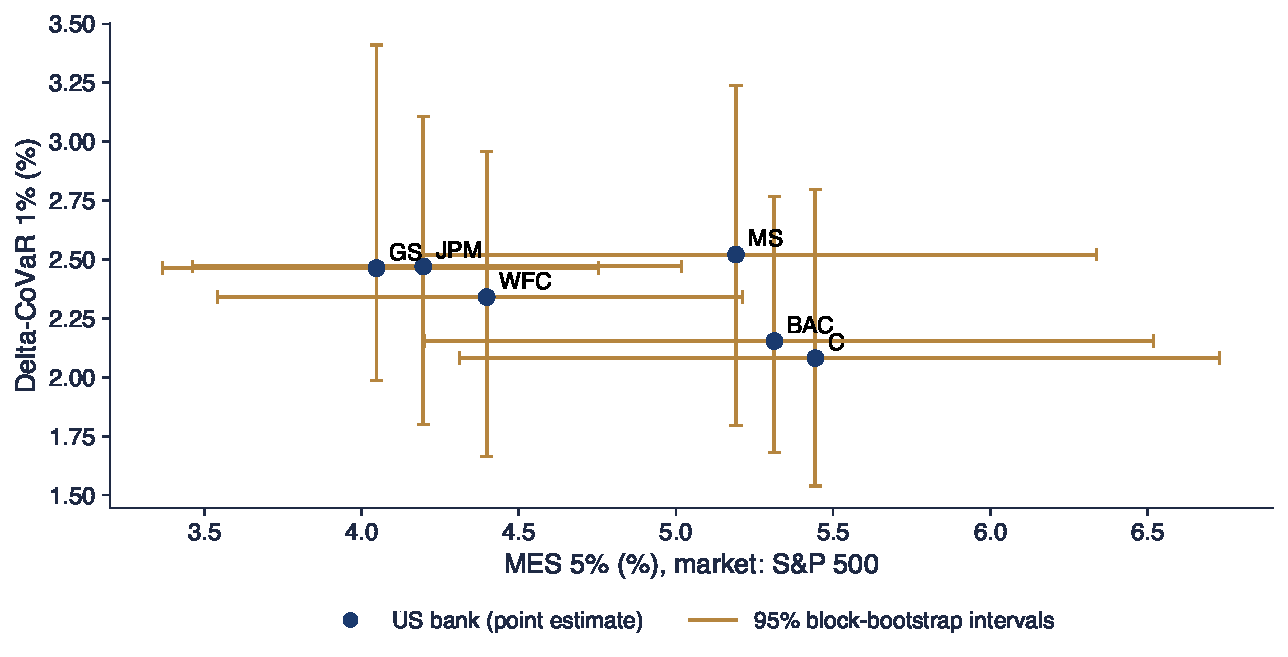
\includegraphics[width=0.96\textwidth,height=0.52\textheight,keepaspectratio]{ch15_sem_b1.pdf}
\end{center}
\vspace{-2mm}
\begin{itemize}
    \item $n = 5\,229$ zile; cel mai mare MES: Citigroup; cel mai mare $\Delta$CoVaR: Morgan Stanley; corelația Spearman a ordonărilor $-0{,}60$
    \item Interpretare: nu: MES pune pe primele locuri băncile care scad cel mai mult odată cu piața (Citigroup, Bank of America), $\Delta$CoVaR băncile a căror criză mișcă cel mai mult piața; intervalele se suprapun, deci niciuna dintre ordonări nu este clară
\end{itemize}\sfmquantlet{Ch_15}{SFM_ch15_seminar}
\end{frame}

\begin{frame}{B2: băncile europene și cele românești [Propus]}
\itemsize{\footnotesize}
\begin{itemize}
\item \textbf{Întrebarea}: apare și în Europa și în România dezacordul dintre MES și $\Delta$CoVaR găsit în B1? Model: B1.
\item \textbf{Date}: cele cinci bănci europene și Euro Stoxx 50 din 2005; TLV, BRD și BET din 2010
\item \textbf{Cerințe}
\begin{enumerate}
    \item Calculați MES 5\% și $\Delta$CoVaR 1\% cu intervale bootstrap pentru fiecare bancă, față de propria piață.
    \item Calculați corelația Spearman a celor două ordonări pentru băncile europene.
    \item Comparați cele două bănci românești după ambele măsuri.
    \item Interpretare: este dezacordul dintre MES și $\Delta$CoVaR la fel de puternic în Europa ca în SUA?
\end{enumerate}
\item \textbf{Raportați}: un tabel și două fraze
\item Notebook: secțiunea B2
\end{itemize}
\end{frame}

\ifsolutions
\begin{frame}{B2: rezolvare [Propus]}
\itemsize{\footnotesize}
\begin{center}
\scriptsize
\begin{tabular}{lrrrr}
\toprule
& MES 5\% & interval 95\% & $\Delta$CoVaR 1\% & interval 95\% \\
\midrule
DBK & $4{,}81$ & [4{,}13; 5{,}49] & $2{,}90$ & [2{,}24; 3{,}83] \\
BNP & $4{,}60$ & [3{,}96; 5{,}29] & $3{,}13$ & [2{,}48; 3{,}67] \\
SAN & $4{,}35$ & [3{,}80; 4{,}95] & $3{,}09$ & [2{,}36; 3{,}82] \\
INGA & $5{,}35$ & [4{,}45; 6{,}33] & $3{,}18$ & [2{,}25; 3{,}90] \\
HSBA & $2{,}90$ & [2{,}47; 3{,}33] & $2{,}87$ & [2{,}14; 3{,}71] \\
\midrule
TLV & $3{,}54$ & [2{,}90; 4{,}24] & $3{,}31$ & [2{,}35; 4{,}78] \\
BRD & $3{,}00$ & [2{,}48; 3{,}70] & $3{,}05$ & [2{,}44; 4{,}12] \\
\bottomrule
\end{tabular}
\end{center}
\begin{itemize}
    \item Europa: cel mai mare MES ING, cel mai mare $\Delta$CoVaR ING; Spearman $0{,}70$; HSBC are de departe cel mai mic MES
    \item România: TLV are MES și $\Delta$CoVaR mai mari, dar intervalele celor două bănci se suprapun mult
    \item Interpretare: nu: în Europa, cele două ordonări sînt mult mai apropiate decît în SUA; băncile sînt mai mari în raport cu Euro Stoxx 50, deci a scădea odată cu piața și a mișca piața merg împreună
\end{itemize}\sfmquantlet{Ch_15}{SFM_ch15_seminar}
\end{frame}
\fi

\begin{frame}{B3: băncile americane și europene în 2008 [Rezolvat]}
\itemsize{\footnotesize}
\begin{itemize}
\item \textbf{Întrebarea}: a devenit mai puternică legătura dintre băncile americane și cele europene după Lehman: contagiune sau interdependență?
\item \textbf{Date}: portofoliile cu ponderi egale ale celor șase bănci americane și cinci bănci europene, zilele comune; perioada calmă: ianuarie 2005 -- iunie 2007; criza: 15 septembrie -- 31 decembrie 2008
\item \textbf{Cerințe}
\begin{enumerate}
    \item Calculați corelația dintre cele două portofolii în perioada calmă și în criză.
    \item Testați creșterea corelației cu testul $z$ unilateral al lui Fisher, la 5\%.
    \item Calculați $\delta$ din varianța portofoliului american și corelația corectată Forbes--Rigobon.
    \item Repetați testul cu corelația corectată.
    \item Interpretare: contagiune sau interdependență?
\end{enumerate}
\item \textbf{Raportați}: șase valori, două decizii, graficul și două fraze
\item Notebook: secțiunea B3
\end{itemize}
\end{frame}

\begin{frame}{B3: rezolvare [Rezolvat]}
\itemsize{\scriptsize}
\begin{center}
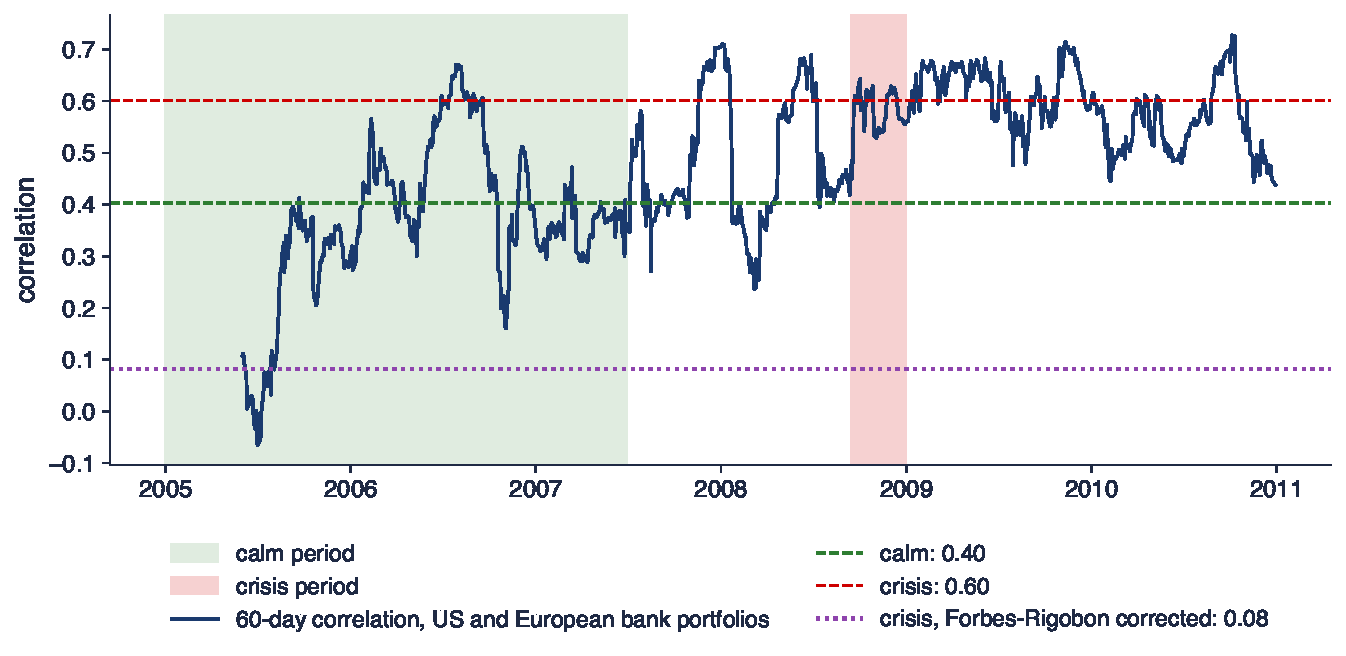
\includegraphics[width=0.96\textwidth,height=0.44\textheight,keepaspectratio]{ch15_sem_b3.pdf}
\end{center}
\vspace{-2mm}
\begin{itemize}
    \item $r_0 = 0{,}40$ ($n_0 = 506$), $r_1 = 0{,}60$ ($n_1 = 72$); $z = (0{,}695 - 0{,}428)/0{,}128 = 2{,}09$, p $= 0{,}018$: creșterea necorectată este semnificativă
    \item Varianța portofoliului american: $0{,}89$ $\to$ $75{,}39$, $\delta = 83{,}68$; $\rho^* = 0{,}60/\sqrt{1 + 83{,}68 \times 0{,}638} = 0{,}08$; $z = -2{,}69$, p $= 0{,}996$: nicio creștere
    \item Interpretare: interdependență: corelația a crescut deoarece varianța băncilor americane a crescut de aproximativ 85 ori; după corecție, legătura nu este mai puternică \refFR
\end{itemize}\sfmquantlet{Ch_15}{SFM_ch15_seminar}
\end{frame}

\begin{frame}{B4: băncile europene și cele românești în 2020 [Propus]}
\itemsize{\footnotesize}
\begin{itemize}
\item \textbf{Întrebarea}: a devenit mai puternică legătura dintre băncile europene și cele românești în prăbușirea din perioada COVID-19? Model: B3.
\item \textbf{Date}: portofoliile cu ponderi egale ale celor cinci bănci europene și ale TLV și BRD, zilele comune din 2010; perioada calmă: 2019; criza: 20 februarie -- 30 aprilie 2020
\item \textbf{Cerințe}
\begin{enumerate}
    \item Calculați corelația în perioada calmă și în criză și testați creșterea cu testul $z$ al lui Fisher.
    \item Calculați $\delta$ din varianța portofoliului european și corelația corectată.
    \item Repetați testul cu corelația corectată.
    \item Interpretare: contagiune sau interdependență?
\end{enumerate}
\item \textbf{Raportați}: șase valori, două decizii și două fraze
\item Notebook: secțiunea B4
\end{itemize}
\end{frame}

\ifsolutions
\begin{frame}{B4: rezolvare [Propus]}
\itemsize{\footnotesize}
\begin{itemize}
    \item $r_0 = 0{,}12$ ($n_0 = 200$), $r_1 = 0{,}70$ ($n_1 = 43$); $z = 4{,}29$, p $< 0{,}001$: creșterea necorectată este semnificativă
    \item Varianța portofoliului european: $2{,}50$ $\to$ $26{,}33$, $\delta = 9{,}52$; $\rho^* = 0{,}70/\sqrt{5{,}90} = 0{,}29$; $z = 1{,}03$, p $= 0{,}152$: nesemnificativ
    \item Interpretare: datele indică interdependență; cu 2019 ca perioadă calmă, corelația a fost neobișnuit de mică, iar cele 43 de zile de criză dau un interval larg, deci testul are o putere redusă
\end{itemize}\sfmquantlet{Ch_15}{SFM_ch15_seminar}
\end{frame}
\fi

\begin{frame}{B5: a ordonat MES din 2019 pierderile din martie 2020? [Rezolvat]}
\itemsize{\footnotesize}
\begin{itemize}
\item \textbf{Întrebarea}: pierd mai mult într-o criză băncile cu MES mare înaintea crizei, ca în \refAPPR?
\item \textbf{Date}: 11 bănci americane și europene; MES 5\% pe randamentele zilnice din 2019; randamentul cumpără-și-păstrează din 19 februarie pînă în 23 martie 2020
\item \textbf{Cerințe}
\begin{enumerate}
    \item Calculați MES 5\% pentru fiecare bancă în 2019, față de propria piață.
    \item Calculați randamentul fiecărei bănci din 19 februarie pînă în 23 martie 2020.
    \item Calculați corelația Spearman dintre MES și randament și p-valoarea ei.
    \item Interpretare: a ordonat MES pierderile din martie 2020?
\end{enumerate}
\item \textbf{Raportați}: graficul, corelația cu p-valoarea ei și două fraze
\item Notebook: secțiunea B5
\end{itemize}
\end{frame}

\begin{frame}{B5: rezolvare [Rezolvat]}
\itemsize{\scriptsize}
\begin{center}
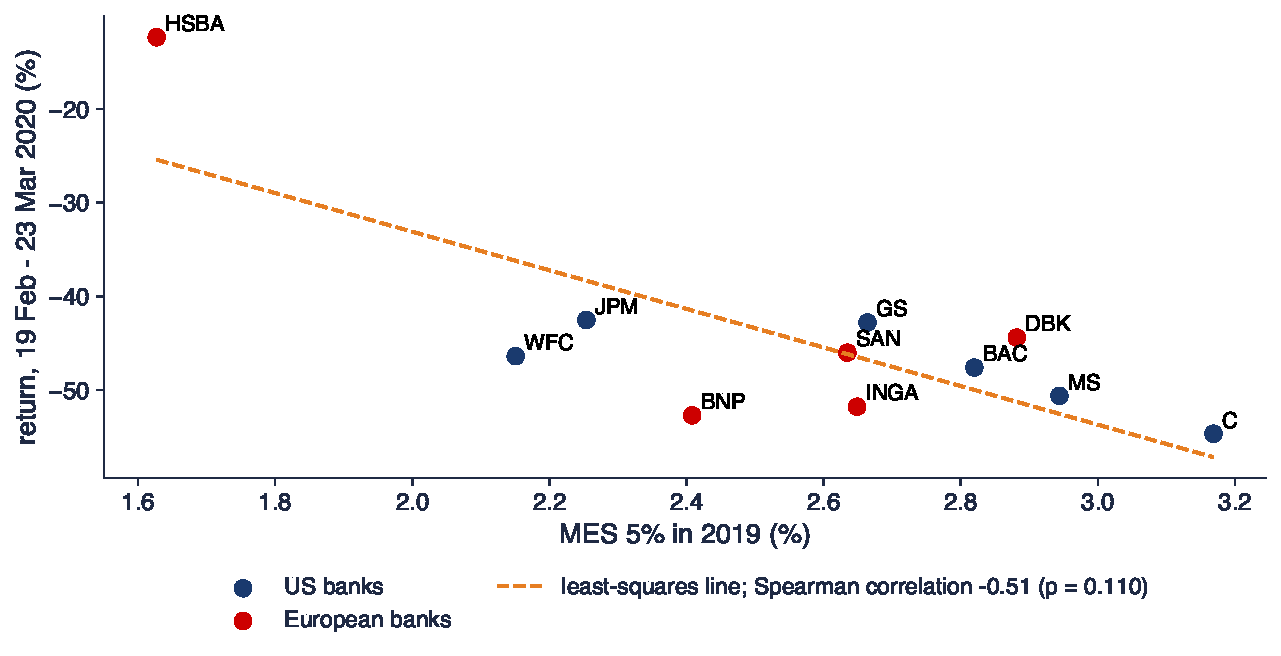
\includegraphics[width=0.96\textwidth,height=0.40\textheight,keepaspectratio]{ch15_sem_b5.pdf}
\end{center}
\vspace{-2mm}
\begin{itemize}
    \item Cel mai mare MES în 2019: Citigroup ($3{,}17\%$), și cel mai prost randament ($-54{,}7\%$); cel mai mic MES: HSBC ($1{,}63\%$), și cea mai mică pierdere ($-12{,}3\%$)
    \item Corelația Spearman $-0{,}51$, p $= 0{,}110$ ($n = 11$)
    \item Interpretare: parțial: semnul este cel din \refAPPR, iar extremele coincid, dar cu 11 bănci corelația nu este semnificativă la 5\%; mijlocul ordonării este zgomot
\end{itemize}\sfmquantlet{Ch_15}{SFM_ch15_seminar}
\end{frame}

\begin{frame}{B6: a ordonat MES din 2022 pierderile din martie 2023? [Propus]}
\itemsize{\footnotesize}
\begin{itemize}
\item \textbf{Întrebarea}: se păstrează rezultatul din B5 în tulburările bancare din martie 2023? Model: B5.
\item \textbf{Date}: 13 bănci (cu TLV și BRD); MES 5\% pe randamentele zilnice din 2022; randamentul din 28 februarie pînă în 31 martie 2023
\item \textbf{Cerințe}
\begin{enumerate}
    \item Calculați MES 5\% pentru fiecare bancă în 2022, față de propria piață.
    \item Calculați randamentul fiecărei bănci din 28 februarie pînă în 31 martie 2023.
    \item Calculați corelația Spearman și p-valoarea ei.
    \item Interpretare: de ce poate MES să nu ordoneze pierderile din martie 2023?
\end{enumerate}
\item \textbf{Raportați}: un tabel, corelația cu p-valoarea ei și două fraze
\item Notebook: secțiunea B6
\end{itemize}
\end{frame}

\ifsolutions
\begin{frame}{B6: rezolvare [Propus]}
\itemsize{\footnotesize}
\begin{center}
\scriptsize
\begin{tabular}{lrr|lrr}
\toprule
Banca & MES 5\% & randament (\%) & Banca & MES 5\% & randament (\%) \\
\midrule
JPM & $2{,}87$ & $-10{,}2$ & BNP & $4{,}71$ & $-16{,}5$ \\
BAC & $3{,}21$ & $-17{,}0$ & SAN & $4{,}21$ & $-8{,}0$ \\
C & $2{,}95$ & $-9{,}1$ & INGA & $5{,}43$ & $-17{,}6$ \\
GS & $2{,}90$ & $-8{,}0$ & HSBA & $2{,}56$ & $-13{,}5$ \\
MS & $3{,}41$ & $-10{,}8$ & TLV & $3{,}37$ & $-0{,}9$ \\
WFC & $3{,}28$ & $-20{,}1$ & BRD & $3{,}99$ & $-10{,}4$ \\
DBK & $5{,}20$ & $-20{,}7$ & & & \\
\bottomrule
\end{tabular}
\end{center}
\begin{itemize}
    \item Spearman $-0{,}35$, p $= 0{,}247$ ($n = 13$); cel mai mare MES: ING; cel mai prost randament: Deutsche Bank
    \item Interpretare: șocul din 2023 a venit din depozite și din riscul de dobîndă al cîtorva bănci (SVB, Credit Suisse), nu dintr-o prăbușire a pieței: MES, construit pe mișcarea comună cu piața, ordonează doar slab un astfel de șoc
\end{itemize}\sfmquantlet{Ch_15}{SFM_ch15_seminar}
\end{frame}
\fi


%=============================================================================
\section{Partea C: întrebări deschise și critica unui răspuns AI}
%=============================================================================

\begin{frame}{C1: cît de conectate sînt băncile românești cu cele din zona euro? [Propus]}
\itemsize{\footnotesize}
\begin{itemize}
\item \textbf{Întrebarea}: ce parte din riscul TLV și BRD vine de la băncile europene și crește această parte în crize?
\item \textbf{Date}: cele cinci bănci europene, TLV și BRD, randamente logaritmice zilnice în zilele comune din 2010; modele: B1, slide-ul despre conectivitate
\item \textbf{Cerințe}
\begin{enumerate}
    \item Estimați un model VAR pe cele șapte serii de randamente (ordinul ales prin BIC) și calculați tabelul de conectivitate pentru $H = 10$ zile.
    \item Calculați proporția din varianța erorii de prognoză a TLV și BRD care vine de la cele cinci bănci europene.
    \item Repetați calculul pe ferestre mobile de 250 de zile și comparați 2019 cu 2020.
    \item Interpretare: este riscul sistemic al băncilor românești importat?
\end{enumerate}
\item \textbf{Raportați}: un tabel și un plan de proiect
\item Notebook: secțiunea C1
\end{itemize}
\end{frame}

\ifsolutions
\begin{frame}{C1: analiză de referință [Propus]}
\itemsize{\footnotesize}
\begin{itemize}
    \item $n = 3\,245$ zile comune, VAR(1); conectivitatea totală a celor șapte bănci 60{,}0\%
    \item Proporția venită de la băncile europene, eșantionul complet: TLV 22{,}9\%, BRD 22{,}1\%
    \item Ferestre mobile de 250 de zile (media TLV și BRD): media 20{,}2\%, 2019 4{,}7\%, 2020 35{,}2\%, maximul 41{,}6\% (fereastra care se încheie la 22 august 2022)
    \item Lectura rezultatelor: în anii liniștiți, aproape tot riscul băncilor românești este local; în crize, o parte mare vine din zona euro
    \item Designul proiectului: ore de tranzacționare diferite (randamente pe două zile), $\Delta$CoVaR cu portofoliul băncilor europene ca variabilă de condiționare, intervale bootstrap pentru proporțiile pe ferestre mobile
\end{itemize}\sfmquantlet{Ch_15}{SFM_ch15_seminar}
\end{frame}
\fi

\begin{frame}{C2: verificați un răspuns AI [Propus]}
\itemsize{\scriptsize}
\begin{itemize}
    \item Un student a cerut unui asistent AI să rezume riscul sistemic al JPMorgan Chase. Răspunsul:
    \item \aiprompt{(a) CoVaR 99\% al S\&P 500 condiționat de JPM este -4{,}80\%.}
    \item \aiprompt{(b) Delta-CoVaR = CoVaR - VaR-ul JPM = 4{,}80 - 6{,}27 = -1{,}48\%, deci JPM reduce riscul sistemic.}
    \item \aiprompt{(c) MES 5\% este pierderea medie a S\&P 500 în cele mai proaste 5\% dintre zilele JPM.}
    \item \aiprompt{(d) Banca cu cel mai mare VaR 1\% este întotdeauna cea mai importantă sistemic.}
    \item \aiprompt{(e) Corelația dintre băncile americane și cele europene a crescut de la 0{,}40 la 0{,}60 în toamna lui 2008, ceea ce dovedește contagiunea.}
    \item \aiprompt{(f) Un SRISK pozitiv înseamnă că banca are mai mult capital decît îi trebuie într-o criză.}
    \item \aiprompt{(g) Cauzalitatea Granger de la banca A la banca B înseamnă că randamentele trecute ale lui A ajută la prognoza lui B; nu dovedește un canal cauzal.}
    \item Cerințe
    \begin{itemize}
        \item 1. Pentru fiecare afirmație, precizați dacă este corectă; dacă nu este, formulați afirmația corectă și, acolo unde se poate, dați valoarea corectă din notebook (secțiunea C2).
        \item 2. Raportați: o listă de șapte verdicte, fiecare cu un rînd de justificare.
    \end{itemize}
\end{itemize}
\end{frame}

\ifsolutions
\begin{frame}{C2: rezolvare [Propus]}
\itemsize{\footnotesize}
\begin{itemize}
    \item (a) Greșit de două ori: nivelul este probabilitatea cozii (CoVaR 1\%), iar CoVaR este o pierdere, un număr pozitiv: CoVaR 1\% $= 4{,}80\%$
    \item (b) Greșit: $\Delta$CoVaR compară CoVaR în dificultate cu CoVaR la mediana JPM: $\Delta$CoVaR 1\% $= 2{,}47\% > 0$ (A1)
    \item (c) Greșit: condiționarea este inversată: MES este pierderea medie a băncii în cele mai proaste zile ale pieței (A3)
    \item (d) Greșit: BAC are un VaR 1\% mai mare decît JPM, dar un $\Delta$CoVaR mai mic (A2)
    \item (e) Greșit: după corecția Forbes--Rigobon, corelația din criză este $0{,}08$: interdependență, nu o contagiune dovedită (B3)
    \item (f) Greșit: SRISK $> 0$ înseamnă capital \textbf{lipsă} într-o criză; un surplus dă SRISK $< 0$ (A5)
    \item (g) Corect
\end{itemize}\sfmquantlet{Ch_15}{SFM_ch15_seminar}
\end{frame}
\fi


%=============================================================================
\section{Încheiere}
%=============================================================================

\begin{frame}{Idei de reținut}
\itemsize{\small}
\begin{itemize}
    \item CoVaR 1\% $= -(\hat a + \hat b\,q_{1\%}(X^i))$ și $\Delta$CoVaR $= \hat b\,(q_{50\%} - q_{1\%})$: sistemul condiționat de bancă
    \item MES: banca condiționată de piață; SRISK $= kD - (1 - k)(1 - \mathrm{LRMES})W$ crește odată cu efectul de levier
    \item VaR, MES și $\Delta$CoVaR ordonează diferit băncile; ordonările au nevoie de intervale bootstrap
    \item O creștere a corelației într-o criză nu este o dovadă de contagiune: corectați pentru volatilitate (Forbes--Rigobon)
    \item Un răspuns AI este o ciornă: verificați nivelul, semnul, direcția condiționării și definiția $\Delta$CoVaR
\end{itemize}
\end{frame}

\begin{frame}{După seminar}
\itemsize{\small}
\begin{itemize}
    \item Cursul 15 dezvoltă fiecare temă de azi: canalele și crizele, CoVaR cu variabile de stare, MES și SRISK, rețele, politica macroprudențială
    \item Încercați cerințele [Propus] în notebook; rezolvările se discută la seminar
    \item C1 poate deveni un proiect de echipă: băncile românești și cele din zona euro, conectivitatea și $\Delta$CoVaR în 2011--2012, 2020 și 2023
    \item Lectură: \refAB; \refAPPR; \refBE; sinteză: \refBCHP
\end{itemize}
\end{frame}


%=============================================================================
\section{Bibliografie}
%=============================================================================

\begin{frame}{Bibliografie}
\itemsize{\tiny}
\begin{itemize}
    \item Acharya, V.V., Engle, R., Richardson, M. (2012). \href{https://doi.org/10.1257/aer.102.3.59}{Capital shortfall: a new approach to ranking and regulating systemic risks}. \textit{American Economic Review}, 102(3), 59--64.
    \item Acharya, V.V., Pedersen, L.H., Philippon, T., Richardson, M. (2017). \href{https://doi.org/10.1093/rfs/hhw088}{Measuring systemic risk}. \textit{Review of Financial Studies}, 30(1), 2--47.
    \item Adrian, T., Brunnermeier, M.K. (2016). \href{https://doi.org/10.1257/aer.20120555}{CoVaR}. \textit{American Economic Review}, 106(7), 1705--1741.
    \item Benoit, S., Colliard, J.-E., Hurlin, C., Pérignon, C. (2017). \href{https://doi.org/10.1093/rof/rfw026}{Where the risks lie: a survey on systemic risk}. \textit{Review of Finance}, 21(1), 109--152.
    \item Brownlees, C., Engle, R.F. (2017). \href{https://doi.org/10.1093/rfs/hhw060}{SRISK: a conditional capital shortfall measure of systemic risk}. \textit{Review of Financial Studies}, 30(1), 48--79.
    \item Diebold, F.X., Yilmaz, K. (2012). \href{https://doi.org/10.1016/j.ijforecast.2011.02.006}{Better to give than to receive: predictive directional measurement of volatility spillovers}. \textit{International Journal of Forecasting}, 28(1), 57--66.
    \item Forbes, K.J., Rigobon, R. (2002). \href{https://doi.org/10.1111/0022-1082.00494}{No contagion, only interdependence: measuring stock market comovements}. \textit{Journal of Finance}, 57(5), 2223--2261.
    \item Franke, J., Härdle, W.K., Hafner, C.M. (2019). \href{https://doi.org/10.1007/978-3-030-13751-9}{\textit{Statistics of Financial Markets: An Introduction}}, 5th ed. Springer.
    \item Granger, C.W.J. (1969). \href{https://doi.org/10.2307/1912791}{Investigating causal relations by econometric models and cross-spectral methods}. \textit{Econometrica}, 37(3), 424--438.
    \item IMF, BIS, FSB (2009). \href{https://www.bis.org/publ/othp07.htm}{Guidance to assess the systemic importance of financial institutions, markets and instruments: initial considerations}. Report to the G-20 Finance Ministers and Central Bank Governors.
    \item Koenker, R., Bassett, G. (1978). \href{https://doi.org/10.2307/1913643}{Regression quantiles}. \textit{Econometrica}, 46(1), 33--50.
\end{itemize}
\end{frame}

\end{document}
